% document class -------------------------------------------
\documentclass[11pt,oneside,openright]{phdthesis}
% ----------------------------------------------------------

\usepackage{float}
\usepackage[linkcolor=black]{hyperref}
\usepackage[sorting=none, backend=biber]{biblatex}
\usepackage[T1]{fontenc}

% graphicx -----------------------------------------------------------------------------------
% The graphicx package allows to specify several paths in which to search for figures.
\usepackage{graphicx}
% --------------------------------------------------------------------------------------------

%\usepackage{amsmath}
%
%
%\usepackage[ansinew]{inputenc}
%%\usepackage[portuguese]{babel}
%\usepackage[printonlyused, withpage]{acronym}
%\usepackage{a4wide}
%\usepackage{palatino}
%\usepackage{fancyhdr}
%\usepackage{fancybox}
%\usepackage{amssymb}
%
%% biblatex ------------------------------------------------------------------------------------------
%% used to divide the bibliography into multiple parts for example per chapter or per section
%\usepackage[sorting=none, backend=biber]{biblatex}
%% ---------------------------------------------------------------------------------------------------
%
%
%\usepackage{epsfig}
%\usepackage{graphics}
%
%\usepackage{here}
%\usepackage{rotating}
%\usepackage{multirow}
%%\usepackage{comment}
%%\usepackage{captionhack}
%\usepackage{epigraph}
%\usepackage[linkcolor=black]{hyperref}
%%\renewcommand{\thesubfigure}{}
%\hypersetup{colorlinks=true}
%\usepackage{enumerate}
%%\usepackage[numbers,sort&compress]{natbib}
%%\usepackage{hypernat}
%\usepackage{booktabs}
%\usepackage{url}                    % needed to cite a site
%\usepackage{eurosym}
%\usepackage{makeidx}
%\usepackage{datatool}
%\usepackage[toc, acronym]{glossaries}
%\usepackage{graphicx}
%\usepackage{caption}
%\usepackage{subcaption}
%
%\usepackage{longtable}				% Multi-page tables
%\usepackage{tabulary}
%\usepackage{braket}
%
%% subfile handling packages
%\usepackage{subfiles}
%
%% For box
%\usepackage{multicol}
%\usepackage{tcolorbox}
%\usepackage{booktabs}
%
%% For flow chart
%\usepackage{tikz}
%\usetikzlibrary{shapes,arrows}
%
%\usepackage{epstopdf}
%\usepackage{listings}
%\usepackage{color}
%\usepackage{textcomp,xcolor}
%
%\usepackage{mathrsfs}
%
%
%% amsfonts ------------------------------------------------------------------------------------------
%% Provides symbols for the number sets (prime, natural, integer, rational, real and complex) in LaTeX
%\usepackage{amsfonts}
%% ---------------------------------------------------------------------------------------------------


\graphicspath{
    {./figures/}
    }

\addbibresource{git_helper.bib}

%
%% my definitions -------------------------------------------
%%\def\bob{}
%\def\dynamicHED{}
%\def\qpsk{}
%\def\optical{}
%\def\bbst{}
%\def\bpsk{}
%\def\dvtxrx{}
%\def\hammingED{}
%\def\huffmanED{}
%\def\arithemeticED{}
%\def\miEstimator{}
%\def\mQAM{}
%\def\lBmQAM{}
%\def\rofKK{}
%\def\dsp{}
%\def\quantumRNG{}
%\def\bb{}
%\def\qokd{}
%\def\dv{}
%\def\quantumA{}
%\def\cvQuantum{}
%\def\qkdCvWithoutBS{}
%\def\intradyne{}
%\def\classicalMpc{}
%\def\quantumMpc{}
%\def\dvQokd{}
%\def\dvQkd{}
\def\etsiQkd{}
\def\secureMPC{}
\def\computationOfPhylogeneticTrees{}
\def\quGenome{}
%\def\secureMultipartyComputationOfPhylogeneticTrees{}
%\def\tinyGarble{}
%\def\aes{}




%% ----------------------------------------------------------
%
%% my packages ----------------------------------------------
%\usepackage{amsmath}
\usepackage{amsfonts}
\usepackage{mathtools}
\usepackage{tabularx}
\usepackage{multirow}

\usepackage{xcolor}


\usepackage[ansinew]{inputenc}
%\usepackage[portuguese]{babel}
\usepackage[printonlyused, withpage]{acronym}
\usepackage{a4wide}
\usepackage{palatino}
\usepackage{fancyhdr}
\usepackage{fancybox}
\usepackage{amssymb}

\usepackage{amsthm}
 \theoremstyle{definition}
 \newtheorem{definition}{Definition}[section]

% biblatex ------------------------------------------------------------------------------------------
% used to divide the bibliography into multiple parts for example per chapter or per section
\usepackage[sorting=none, backend=biber]{biblatex}
% ---------------------------------------------------------------------------------------------------

%\usepackage{chapterbib} %com este package as referencias bibliográficas aparecem no final de cada capítulo
%\usepackage{cite}
\usepackage{epsfig}
%\usepackage{subfigure}
\usepackage{graphics}
\usepackage{float}                   % figures place here [H]
\usepackage{here}
\usepackage[T1]{fontenc}
\usepackage{rotating}
\usepackage{multirow}
%\usepackage{comment}
%\usepackage{captionhack}
\usepackage{epigraph}
\usepackage[linkcolor=black]{hyperref}
%\renewcommand{\thesubfigure}{}
\hypersetup{colorlinks=true}
\usepackage{enumerate}
\usepackage{enumitem}
%\usepackage[numbers,sort&compress]{natbib}
%\usepackage{hypernat}
\usepackage{booktabs}
\usepackage{url}                    % needed to cite a site
\usepackage{eurosym}
\usepackage{makeidx}
\usepackage{datatool}
\usepackage[toc, acronym]{glossaries}

% graphicx -----------------------------------------------------------------------------------
% The graphicx package allows to specify several paths in which to search for figures.
\usepackage{graphicx}
% --------------------------------------------------------------------------------------------

\usepackage{caption}
\usepackage{subcaption}

\usepackage{longtable}				% Multi-page tables
\usepackage{tabulary}
\usepackage{braket}

% subfile handling packages
\usepackage{subfiles}

% For box
\usepackage{multicol}
\usepackage{tcolorbox}
\usepackage{booktabs}

% For flow chart
\usepackage{tikz}
\usetikzlibrary{shapes.geometric,arrows}
\tikzstyle{standard} = [rectangle, rounded corners, minimum width=3cm, minimum height=1cm,text centered, text width=3cm, draw=black]
\tikzstyle{arrow} = [thick,->,>=stealth]

\usepackage{epstopdf}
\usepackage{listings}
\usepackage{color}
\usepackage{textcomp,xcolor}

\usepackage{mathrsfs}


% amsfonts %------------------------------------------------------------------------------------------
% Provides symbols for the number sets (prime, natural, %integer, rational, real and complex) in LaTeX
\usepackage{amsfonts}
%---------------------------------------------------------------------------------------------------
%allows horizontal adjustments on the sections
\usepackage{changepage}
%--------------------------------------------------------------------------------------------------
%For plots with bounds
\usepackage{pgfplots}
\pgfplotsset{compat=1.10}

%--------------------------------------------------------------------
%allows colorful script to the c++ codes
\usepackage{listings}
\usepackage{color}
\definecolor{dkgreen}{rgb}{0,0.6,0}
\definecolor{gray}{rgb}{0.5,0.5,0.5}
\definecolor{mauve}{rgb}{0.58,0,0.82}
\lstset{frame=tb,
  language=c++,
  aboveskip=3mm,
  belowskip=3mm,
  showstringspaces=false,
  columns=flexible,
  basicstyle={\scriptsize\ttfamily},
  numbers=none,
  numberstyle=\tiny\color{gray},
  keywordstyle=\color{blue},
  commentstyle=\color{dkgreen},
  stringstyle=\color{mauve},
  breaklines=true,
  breakatwhitespace=true,
  tabsize=3
}
%--------------------------------------------------------------------

%% ----------------------------------------------------------
%
%% my bib files ---------------------------------------------my
%
%
%%%%%%%%%%%%%%%%%%%%%%%%%%%%%%%%%%%%%%%%%%%%%%%%%%%%%%%%%%%%%%%%%%%%%%%%%%%%%%%%%%%
% Bibliography for the Simulator Structure
%%%%%%%%%%%%%%%%%%%%%%%%%%%%%%%%%%%%%%%%%%%%%%%%%%%%%%%%%%%%%%%%%%%%%%%%%%%%%%%%%%

%\addbibresource{./chapter/simulator_structure/simulator_structure.bib}

%%%%%%%%%%%%%%%%%%%%%%%%%%%%%%%%%%%%%%%%%%%%%%%%%%%%%%%%%%%%%%%%%%%%%%%%%%%%%%%%%%
% Bibliography for SDF
%%%%%%%%%%%%%%%%%%%%%%%%%%%%%%%%%%%%%%%%%%%%%%%%%%%%%%%%%%%%%%%%%%%%%%%%%%%%%%%%%%

\ifdefined\qpsk         \addbibresource{./sdf/qpsk_transmitter/qpsk_transmitter.bib}\fi
\ifdefined\optical      \addbibresource{./sdf/optical_detection/optical_detection.bib}\fi
\ifdefined\bpsk         \addbibresource{./sdf/bpsk_system/bpsk_system.bib}\fi
\ifdefined\m            \addbibresource{./sdf/m_qam_system/m_qam_system.bib}\fi
\ifdefined\simplified   \addbibresource{./sdf/simplified_coherent_receiver/simplified_coherent_receiver.bib}\fi
\ifdefined\dsp          \addbibresource{./sdf/dsp_laser_phase_compensation/dsp_laser_phase_compensation.bib}\fi
\ifdefined\quantumRNG   \addbibresource{./sdf/quantum_random_number_generator/quantum_random_number_generator.bib}\fi
\ifdefined\bb           \addbibresource{./sdf/bb84_with_discrete_variables/bb84_with_discrete_variables.bib}\fi
\ifdefined\bbst         \addbibresource{./sdf/bb84_with_channel_emulator/bb84_with_channel_emulator.bib}\fi
\ifdefined\cvQpskQkd    \addbibresource{./sdf/cv_qpsk_qkd/cv_qpsk_qkd.bib}\fi
\ifdefined\dvtxrx       \addbibresource{./sdf/DvQuantumTxRx/dv_quantum_tx_rx.bib}\fi
\ifdefined\qokd         \addbibresource{./sdf/qokd_with_discrete_variables/qokd_with_discrete_variables.bib}\fi
\ifdefined\dv           \addbibresource{./sdf/dv_polarization_encoding_system/dv_polarization_encoding_system.bib}\fi
\ifdefined\quantumA     \addbibresource{./sdf/quantum_noise/quantum_noise.bib}\fi
\ifdefined\cvQuantum    \addbibresource{./sdf/cv_system/cv_system.bib}\fi
\ifdefined\intradyne    \addbibresource{./sdf/intradyne_cv_system/intradyne_cv_system.bib}\fi
\ifdefined\classicalMpc \addbibresource{./sdf/classical_mpc/classical_mpc.bib}\fi
\ifdefined\quantumMpc   \addbibresource{./sdf/quantum_mpc/quantum_mpc.bib}\fi
\ifdefined\secureMPC    \addbibresource{./sdf/secure_multiparty_computation/secure_multiparty_computation.bib}\fi
\ifdefined\secureMultipartyComputationOfPhylogeneticTrees   \addbibresource{./sdf/secure_multiparty_computation_of_phylogenetic_trees/secure_multiparty_computation_of_phylogenetic_trees.bib}\fi


\ifdefined\miEstimator \addbibresource{./sdf/eit_87071_mutual_information_estimator/eit_87071_mutual_information_estimator.bib}\fi


%%%%%%%%%%%%%%%%%%%%%%%%%%%%%%%%%%%%%%%%%%%%%%%%%%%%%%%%%%%%%%%%%%%%%%%%%%%%%%%%%%
% Bibliography for the library
%%%%%%%%%%%%%%%%%%%%%%%%%%%%%%%%%%%%%%%%%%%%%%%%%%%%%%%%%%%%%%%%%%%%%%%%%%%%%%%%%%

%\addbibresource{./lib/snr_photoelectron_generator/snr_photoelectron_generator.bib}
%\addbibresource{./lib/bit_error_rate/bit_error_rate.bib}
%\addbibresource{./lib/mutual_information_estimator/mutual_information_estimator.bib}

%% ----------------------------------------------------------
%
%% my commands ----------------------------------------------
%\newcommand{\onlyinsubfile}[1]{#1}
\newcommand{\notinsubfile}[1]{}
\renewcommand{\textfraction}{0.01}
\renewcommand{\topfraction}{0.99}
\renewcommand{\floatpagefraction}{0.99}
\renewcommand{\bottomfraction}{0.99}
\renewcommand{\heavyrulewidth}{1pt}
\renewcommand{\lightrulewidth}{0.50pt}
\renewcommand{\chaptername}{Chapter}
\renewcommand{\figurename}{Figure}
\renewcommand{\appendixname}{\Large{Anex}}
\renewcommand{\tablename}{Table}
\renewcommand{\acronymname}{Acronimous}

\newcommand{\mli}[1]{\mathit{#1}}
\newcommand{\intSpace}{\!\!\!\!}
\newcommand{\doubleInt}{\!\!\int\intSpace\int\!\!}
\newcommand{\TX}{\mathit{TX}}
\newcommand{\NLI}{\mathit{NLI}}
\newcommand{\eff}{\mathit{eff}}
\newcommand{\LOASE}{\mathit{LO-ASE}}
\newcommand{\LONLI}{\mathit{LO-NLI}}


%\makesavenoteenv{tabular}



\hyphenpenalty=50000
\tolerance=10000
%%% General page formatting

\oddsidemargin 0.2in
\evensidemargin 0in
%\textwidth 155mm
\headheight 15.0pt
\topmargin 0in
%\textheight 237mm

% footheight 1.0in

\makeatletter
\providecommand*{\diff}%
{\@ifnextchar^{\DIfF}{\DIfF^{}}}
\def\DIfF^#1{%
\mathop{\mathrm{\mathstrut d}}%
\nolimits^{#1}\gobblespace}
\def\gobblespace{%
\futurelet\diffarg\opspace}
\def\opspace{%
\let\DiffSpace\!%
\ifx\diffarg(%
\let\DiffSpace\relax
\else
\ifx\diffarg[%
\let\DiffSpace\relax
\else
\ifx\diffarg\{%
\let\DiffSpace\relax
\fi\fi\fi\DiffSpace}

\providecommand*{\tDeriv}[3][]{%
\frac{\diff^{#1}#2}{\diff #3^{#1}}}
\providecommand*{\pDeriv}[3][]{%
\frac{\partial^{#1}#2}%
{\partial #3^{#1}}}

\graphicspath{{./figures/}{./sdf/bpsk_system/figures/}{./sdf/cv_system/figures/}}


\DeclareMathOperator{\erf}{erf}
\DeclareMathOperator{\erfc}{erfc}
\DeclareMathOperator{\sinc}{sinc}
\DeclareMathOperator{\R}{Re}
\DeclareMathOperator{\I}{Im}
\DeclareMathOperator{\asinh}{asinh}

%\newcommand{\publ}{}

\pagenumbering{arabic} 
%% ----------------------------------------------------------
%
% index ----------------------------------------------------
\makeindex
% ----------------------------------------------------------

\begin{document}

% title -----------------------------------------------------
\title{Git Helper \\ (document under construction)}
\author{Armando Nolasco Pinto}
\date{\today}
\maketitle


% table of contents -----------------------------------------
\tableofcontents
% -----------------------------------------------------------

% -----------------------------------------------------------
%
%% table of contents -----------------------------------------
%\tableofcontents
%% -----------------------------------------------------------

% chapters --------------------------------------------------
%
% ------------------------------------------------------------------------
\chapter{Preface}

Th



%
% ------------------------------------------------------------------------
\chapter{Introduction}

LinkPlanner is devoted to the simulation of point-to-point links.






%
% ------------------------------------------------------------------------
\chapter{Simulator Structure}

LinkPlanner is a signals open-source simulator.

The major entity is the system.

A system comprises a set of blocks.

The blocks interact with each other through signals.

\section{System}

\section{Blocks}

\section{Signals}

List of available signals:

\begin{itemize}
    \item Signal

\end{itemize}









%
% ------------------------------------------------------------------------
\chapter{Development Cycle}

The NetXPTO-LinkPlanner is a open source project implemented using ISO C++.
ISO C++ should be strictly followed in order to increase the portability of the code.

When Visual Studio compiler is used it is recommend to use the \emph{Conformance Mode: /permissive-}, to assure a strick agreement with the ISO C++ standards.

The initial implementation of NetXPTO, September 2016, followed ISO C++14.

The current implementation of NetXPTO, August 2020, follows ISO C++17.

The Git has been used as the version control system.

The NetXPTO-LinkPlanner repository is located in the GitHub site http://github.com/netxpto/linkplanner.
Master branch should be considered a functional beta version of the software.
Periodically new releases are delivered from the master branch under the branch name R<Release Year>-<Release Number>.
The design and integration of the system has been performed by Prof. Armando Nolasco Pinto.

\section{R2020-1}

\begin{enumerate}
    \item {The \emph{using} was not used anymore with unnamed classes.
        Instead unnamed classes were replaced by named classes.
        This change was based on Visual Studio 2019 \href{https://docs.microsoft.com/en-us/cpp/error-messages/compiler-warnings/c5208?view=vs-2019}{Compiler Warning (level 1) C5208 and Error C7626} and on C++ standards committee proposal \href{http://www.open-std.org/jtc1/sc22/wg21/docs/papers/2019/p1766r1.html}{P1766R1};}
\end{enumerate}

\section{Ubuntu Implementation}

Using the executable code in windows on linux, some errors and warnings arise.

The compilation problems found will be presented below, sorted by priority.

\subsection{Organization of Templates} 

The implementation of the templates it must be instantiated in the header file (.h) but with some care to be taken in the source code (.cpp), as it is necessary to make a specific declaration of the model.
In order for the compiler to generate the code, it must see both the template definition (not just declaration) and the specific types/whatever used to "fill in" the template.

If we use the normal implementation of header file and source file, where you put declarations in .h and method definitions in .cpp, and we compile and link the files, it will generate linker errors.The solution is to explicitly instantiate all forms of this model that will be used in this file, as shown in the following example.
\newline
TestClass1.h:
This file contains the class with one template function. It does not contain the template defintion, only the declaration. 

\begin{figure}[h]
	\centering\includegraphics[width=0.5\textwidth]{./sdf/dv_qokd/figures/TesteClass1h.png}
	\caption{TestClass1.h}
	\label{fig:message}
\end{figure}

TestClass1.cpp:
This is where the template is defined, and at the bottom, instanciated explicitly for the types we're going to use in the code.

\begin{figure}[h]
	\centering\includegraphics[width=1\textwidth]{./sdf/dv_qokd/figures/TesteClass1cpp.png}
	\caption{TestClass1.cpp}
	\label{fig:message}
\end{figure}

\vspace{4cm}

TestClass2.h:

\begin{figure}[h]
	\centering\includegraphics[width=0.4\textwidth]{./sdf/dv_qokd/figures/TesteClass2h.png}
	\caption{TestClass2.h}
	\label{fig:message}
\end{figure}

TestClass2.cpp:

\begin{figure}[h]
	\centering\includegraphics[width=0.6\textwidth]{./sdf/dv_qokd/figures/TesteClass2cpp.png}
	\caption{TestClass2.cpp}
	\label{fig:message}
\end{figure}

main.cpp:
\begin{figure}[h]
	\centering\includegraphics[width=0.6\textwidth]{./sdf/dv_qokd/figures/main.png}
	\caption{main.cpp}
	\label{fig:message}
\end{figure}



\subsection{Compilation Problems} 
On Ubuntu 18.04 LTS with version c++17.

Function netxpto\_linux\_20190816.cpp

\begin{enumerate}	
	\item \textbf{warning:} comparison of integer expressions of different signedness: 'int' and 'std::vector<std::complex<double> >::size\_type' \{aka 'long unsigned int'\} [-Wsign-compare]
	2104 |  for (int i = 0; \textbf{i != vec.size();} ++i)
\end{enumerate}

Header File netxpto\_linux\_20190816.h:

\begin{enumerate}
	\item \textbf{warning:} 'Signal::fileName' will be initialized after [-Wreorder]
	361 |  std::string \textbf{fileName}\{ "" \};
	
	\item \textbf{warning:} narrowing conversion of 'bLength' from 't\_unsigned\_long' \{aka 'long unsigned int'\} to 't\_unsigned' \{aka 'unsigned int'\} [-Wnarrowing]
	249 |  explicit Signal(std::string fileName, t\_unsigned\_long bLength) : fileName\{ fileName \}, bufferLength\{ \textbf{bLength} \}, saveSignal\{ true \} \{\};
	
	\item \textbf{warning:} 'Signal::folderName' will be initialized after [-Wreorder]
	362 |  std::string \textbf{folderName}\{ "signals" \};
	
	\item \textbf{warning:} deleting 'void*' is undefined [-Wdelete-incomplete]
	255 |  virtual ~Signal() \{ if ( buffer != nullptr ) \{ delete(buffer); \} \}
	
	\item \textbf{warning:}	'bool Signal::saveSignal' [-Wreorder]
	354 |  bool \textbf{saveSignal}\{ false \};
	
	\item \textbf{warning:} when initialized here [-Wreorder]
	248 |  explicit \textbf{Signal}(std::string fileName) : fileName\{ fileName \}, saveSignal\{ true \} {};
	
	\item \textbf{warning:} when initialized here [-Wreorder]
	249 |  explicit Signal(std::string fileName, t\_unsigned\_long bLength) : fileName\{ fileName \}, bufferLength\{ \textbf{bLength} \}, saveSignal\{ true \} \{\};
	
	\item \textbf{warning:} 'Signal::folderName' will be initialized after [-Wreorder]
	362 |  std::string \textbf{folderName}\{ "signals" \};        // folder where signals are going to be saved by default
	
	\item \textbf{warning:} 'const t\_unsigned Signal::bufferLength' [-Wreorder]
	348 |  const t\_unsigned \textbf{bufferLength}\{ DEFAULT\_BUFFER\_LENGTH \};  // Buffer length
	
	\item \textbf{warning:} when initialized here [-Wreorder]
	250 |  explicit \textbf{Signal}(std::string fileName, std::string folderName) : fileName\{ fileName \}, folderName\{ folderName \}, saveSignal\{ true \} \{\}
	
	\item \textbf{warning:} narrowing conversion of 'bLength' from 't\_unsigned\_long' \{aka 'long unsigned int'\} to 't\_unsigned' \{aka 'unsigned int'\} [-Wnarrowing]
	252 |  explicit Signal(t\_unsigned\_long bLength) : bufferLength\{ \textbf{bLength} \} \{\};
	
\end{enumerate}


%\include{chapter/visualizer}
%
% ------------------------------------------------------------------------
\chapter{Case Studies}

\ifdefined\etsiQkd        
\clearpage\clearpage
\graphicspath{{sdf/key_management_layer/figures/}}
\acresetall

\section{Key Management Layer}
% Show subsubsections on the Table of Contents
\setcounter{tocdepth}{4}
\setcounter{secnumdepth}{4}

\begin{refsection}
	\begin{tcolorbox}
		\begin{tabular}{p{2.75cm} p{0.2cm} p{10.5cm}}
			\textbf{Goal}          &:& Design and implementation of a quantum key management layer\\
			\textbf{Directory}     &:& sdf/key\_management\_layer\\
			\textbf{Contributors}   &:& Armando Nolasco Pinto (2023/03/-- ----/--/--) \\
									&& Diogo Matos (2023/03/14 - ----/--/--) \\
		\end{tabular}
	\end{tcolorbox}

%%%%%%%%%%%%%%%%%%%%%%%%%%%%%%%%%%%%%%

\subsection{Introduction}

Quantum Key Distribution (QKD) enables the negotiation of cryptographic keys in a secure manner without relying on computational complexity to achieve its security. On top of the QKD systems a \ac{KML} need to exist in order to mediate the key provisioning to the applications. The key manager provides keys with characteristics requested by the apps and bond to a pre-negotiated quality of service. The proposed system follows Discretion's and ETSI standards [1][2][3]. The system differentiates itself in the fact that mostly (or only) receives quantum oblivious keys from the QKD devices. A future version of the key manager should be able to offer classical, post-quantum and quantum keys, helping its integration into existing networks and providing more flexibility to its clients.

%%%%%%%%%%%%%%%%%%%%%%%%%%%%%%%%%%%%%%

\subsection{Notes and considerations}
\begin{itemize}
	\item During this section, quantum oblivious keys will be divided into two types, A and X. In any connection involving a oblivious keys, one of the parties will receive keys of type A and the other of type X. Keys of type A are whole keys, and keys of type X are keys that are a representation, in a oblivious key fashion, of half of its respective type A key.
	\item In this first version, only the quantum part of the system is specified, though it's our intention to support classical and post-quantum keys too. Nevertheless the system from scratch should be modular enough to facilitate this integration. 
	\item This section will be gradually updated even during the implementation of the system. Some dependencies, like the SDN Agent and the QKD Devices, and issues only found during the implementation might trigger the need to change/enrich this specifications. 
\end{itemize}

%%%%%%%%%%%%%%%%%%%%%%%%%%%%%%%%%%%%%%

\subsection{Architecture}

\begin{figure}[H]
	\centering
	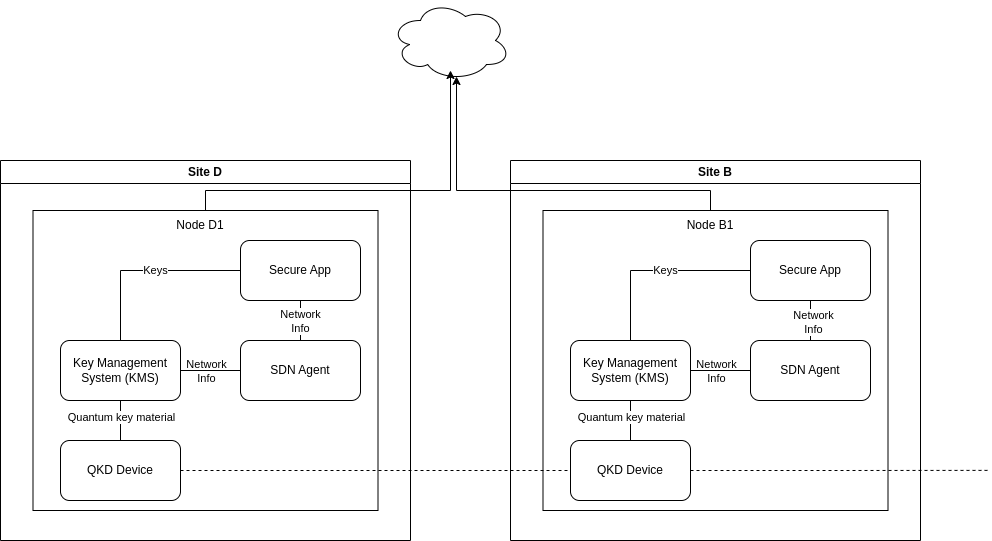
\includegraphics[width=15cm]{kml_arch.png}
	\caption{System architecture}
	\label{fig:kmlarch}
\end{figure}

In the diagram above (\autoref{fig:kmlarch} a simple overview over the whole system in a two node scenario where the \ac{KMS} is integrated can be seen. The dashed line represents a quantum link and the cloud is the black network where, for example, the \ac{SDN} Controller is located. Each secure site have one or more SD-QKD nodes each identified by its \textit{qkdn\_id}. More information on SD-QKD nodes, QKD interfaces, QKD key association links can be found in the standard ETSI QKD 015 [2]. The \ac{KMS} is connected to a physical layer that provides keys to it. These keys can be symmetrical or oblivious and can be generated in distinct manners - classical, post-quantum or quantum (our main focus). Multiple applications are connected to it in order to retrieve keys. Both interfaces, to the applications and to the QKD devices, are based on ETSI QKD 004 standard [1]. Each KMS is connected to at least one KMS that is considered to be its peer since they receive matching keys from the physical layer. Also, the \ac{SDN} agent (\ac{SDN} Controller representative inside the node) is connected to the \ac{KMS} and is used, from the \ac{KMS} perspective, to retrieve information about the network, provide QoS parameters and to receive command orders.

The type of key sources connected to the \ac{KMS} might limit the keys that this one can provide. The connection to a oblivious key source is enough to provide both symmetrical and oblivious keys and even random numbers. Though the key rate might be lower because in order generate a symmetrical key using oblivious keys, twice of the size of wished key will be used.

\begin{figure}[H]
	\centering
	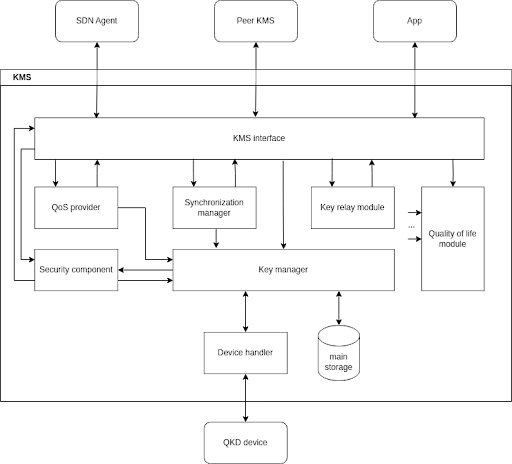
\includegraphics[width=10cm]{kms_modules.png}
	\caption{\ac{KMS} logical modules}
	\label{fig:kmsmodules}
\end{figure}

Apart from just receiving and sending keys through its South and North bound interfaces respectively, the \ac{KMS} need to store, maintain, synchronize, derive and relay (forward) keys. The \ac{KMS} is divided into various logical modules (\autoref{fig:kmsmodules}), namely:

\begin{itemize}
	\item{ \underline{KMS interface (north bound interface)}} 
	
	ETSI QKD 004 based interface to the applications(see \ref{kms_api_apps}). Interface to the \ac{SDN} Agent (to be defined) and to its peer \ac{KMS}s.
	
	\item{\underline{QoS provider}} 
	
	Gathers and provides all QoS parameters to be used to negotiate with the applications and to send them to the \ac{SDN} Agent when requested.
	
	\item{\underline{Synchronization manager}} 
	
	Handles the synchronization protocol (see \ref{key_synch})
	
	\item{\underline{Security component}} 
	
	Implements all cryptographic algorithms used during the operation of the \ac{KMS}.
	
	\item{\underline{Key relay module}} 
	
	Handles the key relay(forwarding) process (see \ref{kms_key_relay}).
	
	\item{\underline{Key manager}} 
	
	Maintains and handles keys. Is mainly used for key material retrieval, storage, etc. It's involved in almost any activity related with keys.
	
	\item{\underline{Base functionality}} 
	
	Handles several quality-of-life features such as logging and configuration.
	
	\item{\underline{Device handler}} 
	
	Handles devices connected to the \ac{KMS} (such as the QKD devices).

\end{itemize}


%%%%%%%%%%%%%%%%%%%%%%%%%%%%%%%%%%%%%%

\subsection{KMS interface to the apps}
\label{kms_api_apps}
This interface follows the ETSI QKD 004 [1] standard in pull mode, it was presented before in \ref{etsi_004} where more detailed information can be found, nevertheless here is made a brief overlook of the API. During the implementation all error cases should be considered and handled has defined in the standard.

\vspace{5mm}

The interaction between \ac{KMS} and app is based on three request, namely:

\begin{lstlisting}
	OPEN_CONNECT(in source, in destination, inout QoS, inout Key_stream_ID, out status)
	GET_KEY(in Key_stream_ID, inout index, out Key_buffer, inout Metadata, out status)
	CLOSE(in Key_stream_ID, out status)
\end{lstlisting}

The OPEN\_CONNECT request is made by an app to create a key stream with the characteristics specified in the QoS field. A \ac{KSID} is returned. If the OPEN\_CONNECT request is made with a value in the Key\_stream\_ID field, it connects to an existing Key Stream instead of creating a new one. 

The GET\_KEY request is used by the apps to retrieve keys. It can be made with or without an index. With a given index, the \ac{KMS} will return the key, if exists, with that index. Otherwise, it return the oldest key that was created by its peer by not retrieved yet, if there is no keys to be return, a new one will be created and returned alongside with its index.

The CLOSE request is used to terminate a Key Stream connection. The peer still can retrieve already created and unexpired keys.

\vspace{5mm}

Since the proposed system is able to offer different types of keys, to the Quality of Service field in the OPEN\_CONNECT was added one extra parameter called 'Key\_type'. After the changes, the QoS parameters are:
		
\begin{itemize}
	\item{\underline{Key\textunderscore type}}
				
	Key type for the key stream. 0: classical symmetrical, 1: P.Q. symmetrical, 2: quantum symmetrical, 3/4: classical oblivious (A/X), 5/6: P.Q. oblivious (A/X), 7/8: quantum oblivious (A/X).
				
	\item{\underline{Key\textunderscore chunk\textunderscore size}}
				
	Length of the key buffer requested by the application. 32 bit unsigned integer.
				
	\item{\underline{Max\textunderscore bps}}
			
	Maximum key rate requested in bits per seconds. 32 bit unsigned integer.
				
	\item{\underline{Min\textunderscore bps}}
			
	Minimum key rate requested in bits per seconds. 32 bit unsigned integer.
				
	\item{\underline{Jitter}}
				
	Maximum expected deviation, in bps, for key delivery. 32 bit unsigned integer.
	
	\item{\underline{Timeout}}	
	
	Time, in msec, after which the all will be aborted, returning an error.
			
	\item{\underline{TTL (Time to Live)}}
			
	Time after which the keys corresponding to this Key\textunderscore stream\textunderscore ID shall be erased. 32 bit unsigned integer.
				
	\item{\underline{Metadata mimetype}}
			
	Field that defines the format of the metadata on each subsequent GET\textunderscore KEY call. Char array of size 256. JSON by default.
				
		\end{itemize}

%%%%%%%%%%%%%%%%%%%%%%%%%%%%%%%%%%%%%%		
		
\subsection{South bound interface (interface to the physical layer)}		

In order for the \ac{KMS} to provide keys to the applications, it first needs to receive key material from the physical layer (a set of QKD devices). The interface between those two is based on ETSI QKD 004 [1] in push mode (the KMS is always receiving keys without making individual requests for each one). This interface is basically the same as the one provided by the KMS for the applications to use but now the \ac{KMS} will act like an application requesting key material. The QoS parameters are the ones defined by ETSI's since usually each QKD device can only provide one key type. The KMS will start by making an OPEN\_CONNECT request to create a connection to the QKD device. Then does one GET\_KEY request and from that moment forward it will receive key material with the characteristics and pace specified in the QoS field until it makes a CLOSE request to terminate the key stream. The \ac{QKD} device provide key material to the \ac{KMS} by continuously sending key\_buffers with its respective metadata. 

%%%%%%%%%%%%%%%%%%%%%%%%%%%%%%%%%%%%%%

\subsection{KMS interface to the SDN Agent and app registration}
\label{kms_agent}	

Every time a new application, any entity requesting keys, connects to the \ac{KMS}, it needs to be  properly registered. The existence of all applications and properties inside the QKD network is only known by the SDN Controller. The following steps need to be made after a OPEN\_CONNECT request from an application to the \ac{KMS}:
\begin{enumerate}
	\item Before any further action, the QoS parameters need to be checked, if the \ac{KMS} cannot provide the QoS proposed by the application, it responds with a status code equal to 7 (OPEN\_CONNECT failed because requested QoS settings could not be met, counterproposal has been included). This process repeats until both agree on a specific QoS.
	\item The SD-QKD node (the \ac{KMS} in this case), as it does not have information about the peer application or its SD-QKD node (remote), informs the SDN controller, via the SDN agent, of this new request, forwarding the same information as in the application request (Src app, Dst app, QoS), also including the local SD-QKD node ID.
	\item If the peer application is not yet registered in the SDN controller, the controller sends back an acknowledgement, but without further information of the peer SD-QKD node. As specified in ETSI QKD 004 [1] an OPEN\_CONNECT blocks, with a threshold defined in the timeout parameter in the QoS, until both applications are connected. If the peer is already connected, move to point number 5.
	\item In the other secure node, the peer application connects to the \ac{KMS}. The SD-QKD node does not have the peer application or SD-QKD node information, so it informs the SDN controller, via the SDN agent, of the incoming application and its requirements.
	\item Now with both applications connected and registered, the SDN controller detects it, created a globally unique \textit{app\_id} (also known as \textit{ksid} to the \ac{KMS}), and sends to both SD-QKD nodes all the necessary information to configure the application at each endpoint (applications and nodes IDs, the \textit{app\_id} and the QoS requirements).
\end{enumerate}

This process is for when the nodes have a physical quantum link, otherwise the process would have some slight differences that are explored in \ref{kms_key_relay}. 

\vspace{5mm}

The specification of the SDN Controller and Agent is out of the scope of this section, but an interface between the \ac{KMS} and the SDN Agent is starting to get some shape just in order to correctly carry out the process described above.

\begin{table}[h!]
\centering
\begin{tabular}{|p{0.2\textwidth} | p{0.1\textwidth} | p{0.1\textwidth} | p{0.2\textwidth} | p{0.3\textwidth}|} 
 \hline
 Name & From & To & Arguments & Notes \\
 \hline\hline
 NEW\_APP & KMS & SDN Agent & Src, Dst, QoS, Node\_id & Replied with a REGISTER\_APP or an acknowledge with a status code informing that the peer application is not connected \\
 \hline
 REGISTER\_APP & SDN Agent & KMS & Src, Dst, QoS, Node\_src, Node\_dst, app\_id & None \\
 \hline
\end{tabular}
\caption{KMS/SDN Agent requests related to application registration.}
\label{table:1}
\end{table}

Additionally, the KMS should be able to be configured by the SDN Controller. Mainly for creation, modification and deletion of links. The manipulation of logical links is crucial for the process of key forwarding (\ref{kms_key_relay}).



%%%%%%%%%%%%%%%%%%%%%%%%%%%%%%%%%%%%%%	
\subsection{Key storage}
\label{key_storage}

All keys are stored in a \ac{DB} that's accessed by the key manager in order to create and retrieve keys. As most as possible the \ac{DB} should have mechanisms to create an abstraction layer, such as stored procedures and triggers, making it more resilient, secure and self sustaining. This same \ac{DB} might be used to save other useful information as connected devices, application information and a basic network topology.

\begin{figure}[H]
	\centering
	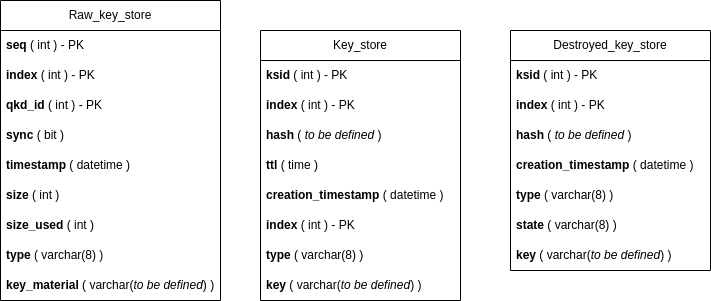
\includegraphics[width=15cm]{db.png}
	\caption{Database entity relationship diagram}
	\label{fig:dberd}
\end{figure}

As can be seen in diagram above (\autoref{fig:dberd}), the \ac{DB} is divided into three main tables. 

The \textit{Raw\_key\_store} has key material as received from the physical layer. This key material is not considered internally to be a already created key, instead will be used in the future to create keys when requested by the applications. This table is organized into the following fields:
\begin{itemize}
	\item seq (int)(PK) - Sequence number attached to the frame sent by the QKD device.
	\item index (int)(PK) - Index of the key material chunk after being split. The size of the data field in the frames sent by the QKD devices is variable, so it might be too large to or inconvenient to store it all in one entry in the \ac{DB}.
	\item qkd\_id (int)(PK) - QKD device identifier. 
	\item sync (bit) - Boolean value that tells if the key material is in sync with the peer.
	\item timestamp (datetime) - Date and time of when key material was save.
	\item size (int) - key material size in bytes.
	\item size\_used (int) - number of bytes already used.
	\item type (int) - key type. 0: classical symmetrical, 1: P.Q. symmetrical, 2: quantum symmetrical, 3/4: classical oblivious (A/X), 5/6: P.Q. oblivious (A/X), 7/8: quantum oblivious (A/X). 
	\item key\_material (varchar(4096)) - key material.
\end{itemize}

The table shall have a maximum number of rows, after the table is full new keys must be discarded. Let say that the maximum is set to one million entries, the \ac{DB} can store about 4 Gb of raw key material. Both this value and the maximum size of the key material might be changed depending on expected the key rate and the key material sent by the physical layer.

\vspace{5mm}

The \textit{Key\_store} table has the created keys. This table should have at least the following fields:
\begin{itemize}
	\item ksid (int)(PK) - Key stream id that the key is related to. For internal keys, set to the symmetric value of the id of the peer KMS which the key is shared.
	\item index (int)(PK) - index of the key in the context of the key stream (sequential).
	\item hash (tbd) - hash value or some kind of checksum used in order to check the integrity of the key with the peer \ac{KMS}.
	\item expiration\_timestamp (datetime) - Expiration date. 
	\item suspended (bit) - boolean value that tells if the key is in the suspended state.
	\item creation\_timestamp (datetime) - Timestamp of when the key was created.
	\item type (int) - Key type. Classical oblivious (A/X), 5/6: P.Q. oblivious (A/X), 7/8: quaSntum oblivious (A/X).
	\item used (bit) - Boolean value that tells if the keys was already given to the app. It's used in order for a GET\_KEY request is made without a given index and the the oldest key not provided yet should be returned is exists.  
	\item key\_material - key material. 
\end{itemize}

\vspace{5mm}

The final table related to keys is the \textit{Deleted\_key\_store} that its only purpose is to reduce the size of the \textit{Key\_store} by moving keys in the deleted state to this table.

\vspace{5mm}

Any key created has to go through its life-cycle. The states and timings are specified by NIST(NIST SP 800-57) and a summary of the standard can be found \href{https://cloud.ibm.com/docs/key-protect?topic=key-protect-key-states}{here}. The key state can be extracted from the \textit{expiration\_timestamp} and \textit{creation\_timestamp}. The only state that cannot be derived from the timestamps is the suspended mode, for that purpose the \textit{suspended} parameter in the \textit{Key\_store} table is used.

\vspace{5mm}

In terms of the mechanisms to keep the database to a certain degree clean, at least two scheduled events (scripts that run periodically) should be deployed in the \ac{DB} - one to delete old not synced keys from the \textit{Raw\_key\_store} and other to move keys to \textit{Destroyed\_key\_store} based on the timestamps.

%%%%%%%%%%%%%%%%%%%%%%%%%%%%%%%%%%%%%%	

\subsection{Key synchronization}
\label{key_synch}

The keys stored by peer \ac{KMS}s have to match, not necessarily be identical, in order to correctly providing them to the applications. A key is synchronized if both peers have received it and both are aware of that fact.

A \ac{KMS} to inform its peer of what keys it has received from the physical layer, a \textit{key\_synch} message is sent with a set of \textit{index}s of the keys received since the last message of the same type. The number of \textit{index}s in one message it may vary from KMS to KMS, as an example a \ac{KMS} with a higher key rate might have a higher number of SEQ\_ID's per message. For this process to work properly the \textit{Key\_chunk\_size} agreed on between each KMS and the respective QKD device need to be same, otherwise it's impossible to synchronize the keys using this method.

\vspace{5mm}

Each time a new key\_buffer is received by a KMS, an action will be performed based on the following criteria:
\begin{itemize}
\item current index  was mentioned in a KEY\_SYNC message sent by the peer KMS, and the number of distinct indexs was reached in order to send a KEY\_SYNC message:
	
action: send KEY\_SYNC message to peer including the last received index and store key material with sync field at 1 (true).

\item current index was not mentioned by its peer KMS’s KEY\_SYNC messages and the last notified seq is higher than the current seq:

action: discard keys

\item default:

action: store keys with sync field at 0 (false)
\end{itemize}

The sync field of a key in the \textit{raw\_key\_store} might be updated later based on the received \textit{key\_synch} messages. In order to set it to 1, both the following conditions need to be checked:
\begin{enumerate}
	\item A KEY\_SYNC message was received from the peer with the index of the key material associated with the key.
	\item The \ac{KMS} has sent a \textit{key\_synch} message notifying the peer the reception of the key material from where the key was took. 
\end{enumerate}

Not synced keys should be discarded after a high enough time period for a well functioning \ac{KMS} to send at least one \textit{key\_synch} message. The value of this time period must be configurable. The removal of keys from the \ac{DB} is made by a routine programmed in the \ac{DB} that runs periodically (see \ref{key_storage}).

%%%%%%%%%%%%%%%%%%%%%%%%%%%%%%%%%%%%%%

\subsection{Key relay}
\label{kms_key_relay}

Since the QKD devices only generate matching key material between two directly connected devices, but matching keys are required to be present at two arbitrary nodes, a process to take a key from a \ac{KMS} to other \ac{KMS} (from a node to another node) not directly connected need to be available. A QKD Key Association Link is a logical key association between two remote SD-QKD nodes, each one being of one of two types: direct, if there is a quantum channel connecting the nodes, or virtual if keys are forwarded(key relay) through multiple trusted nodes to form an end-to-end association.

The key relay process, the creation and configuration of virtual links, is managed by the SDN Controller and the key relay is performed by a set of \ac{KMS}s. The KMS / SDN Agent interaction during this process is not much specified in the standards (ETSI QKD 004 [1] and 015 [2]), though we know that each relay node is configured with the previous and next node in the path, the respective \textit{ksid} and relay method to be used. In some specific cases where there is redundant direct links between nodes, it might also specify the link for the relay. This configuration is done between the NEW\_APP and APP\_REGISTRATION requests (see \ref{kms_agent}). Those properties are used by the SDN Agent to configure the \ac{KMS}.

\vspace{5mm}

\begin{figure}[H]
	\centering
	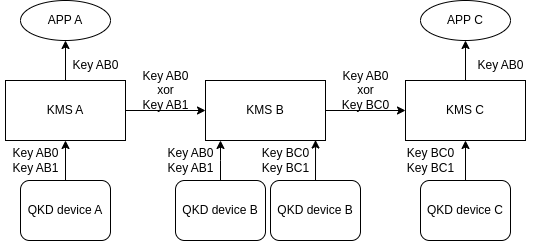
\includegraphics[width=15cm]{key_relay.png}
	\caption{Key relay process}
	\label{fig:keyrelay}
\end{figure}

The basic key relay method (see \autoref{fig:keyrelay}) is done by using \ac{OTP} performing a XOR between the key to be relayed and a key that both peer \ac{KMS}s know, this operation is done each hop. This key relay method requires all nodes to be trusted,  in some specific cases that might be a problem. In a future implementation of the system more relay method can be added and used based on the security requirements on each end-to-end connection. Some other methods can be found in ETSI QKD 014 [4] and in this paper [5].

%%%%%%%%%%%%%%%%%%%%%%%%%%%%%%%%%%%%%
\subsection{Communication between KMSs}
\label{kms_com}

The communication directly between peer \ac{KMS}s is done over a low fidelity channel used only for synchronization purposes. There's two types of massages, namely:

\begin{itemize}
	\item NEW\_KEY
		\begin{itemize}
			\item \textbf{Parameters} - Key Stream Id (Ksid), index, hash
			\item \textbf{Goal} - Establish the creation of a key.
			\item \textbf{Observations} - The peer KMS should create the key too and acknowledge it. The KMS that sends this message should only create the key after receiving the acknowledgement. If the message is not acknowledge during a valid time period (timeout defined in the QoS field in the OPEN\_CONNECT request) no key should be created. The \textit{index} field is not the index of the key to be created but the index of the raw key material from where the key will be extracted and it's optional.
		\end{itemize}
	\item NEW\_INTERNAL\_KEY
		\begin{itemize}
			\item \textbf{Parameters} - index, hash
			\item \textbf{Goal} - Establish the creation of a key to be used internally by both peer KMSs. Usually, this keys are used for authentication and integrity check of messages when communicating with each other.
		\end{itemize}
	\item KEY\_SYNC 
		\begin{itemize}
			\item \textbf{Parameters} - Received key indexs (received\_indexs)
			\item \textbf{Goal} - Notify peer of what key material it was received from the physical layer. See \ref{key_synch}.
		\end{itemize}
	\item KEY\_RELAY
		\begin{itemize}
			\item \textbf{Parameters} - Multiple encrypted keys, their respective IDs and the ID of the relay process (used to know the next hop)
			\item \textbf{Goal} - Forward keys to the next hop in the key relay process enabling key share between two not directly connected nodes. 
		\end{itemize}
\end{itemize}

%%%%%%%%%%%%%%%%%%%%%%%%%%%%%%%%%%%%%%
\subsection{Quality of service providing}
In order for the QKD network to work effectively, the SDN Controller need to be aware of some basic QoS parameters of the \ac{KMS}. The \ac{KMS} at any point can receive a request from the SDN Agent asking for the current QoS metrics, for that the \ac{KMS} has a dedicated module (QoS provider) that keeps a updated set of metrics of the current state of the system. This parameters are not specified explicitly in the specifications, but some can be extracted from some of the operations done by the SDN Controller like the proposed optimal key relay path computation algorithm. Each QoS parameter that might vary from key type to key type (e.g. key\_availability) must be provided such way that distinction can be made. For now, the QoS metrics are:

\begin{itemize}
	\item \underline{key\_availability}
	
	Total size of key material ready to be used (in bytes).
	
	\item \underline{key\_rate}	
	
	Rate at which keys are received from the QKD devices. 
	
	\item \underline{effective\_key\_rate}	
	
	Rate at which keys can be provided to an application (in bps). Does not include key that are used internally by the KMS.
	
	\item \underline{average\_key\_consuption\_per\_link}	
	
	Average key consumption (in bps). Very useful to compute optimal paths (in bps).
	
\end{itemize}

%%%%%%%%%%%%%%%%%%%%%%%%%%%%%%%%%%%%%%
\subsection{Algorithm security}
To assure \ac{ITS} of the system as a whole, every module need to use \ac{ITS} algorithms to promise security against an adversary with unbound computational power. 

\subsubsection{Authentication and integrity}
Can be achieved by using a \ac{MAC}, such as UMAC or Poly1305. Both the transmitter and the receiver have a shared secret, used by the first to create the \ac{MAC} and by the other to verify the authenticity of the sender and the integrity of the message. This must be used in all communication where is possible to have shared keys, such between KMSs where it can take an advantage from QKD. But in order to assure both this aspect in a communication such as between the KMS and a secure app the use of asymmetrical algorithms would be perfect to bypass the QKD, but classical \ac{KEM} is not IT secure. The use of post-quantum and hybrid algorithms could be used to authenticate and share a keys between them. There's a very limited amount of \ac{ITS} post-quantum algorithms, right now being advised to use hybrid algorithms instead. The use of certificates would simplify authentication and authorization allowing all entities in the system to identify themselves and others.

\subsubsection{Encryption}
Encryption is most importantly used in the communication between KMSs since all data is transmitted over the black network. Idealizing the use of QKD shared keys, the encryption of data can be as simple as a XOR, that is IT secure as long a different key is always used and its size it's equal to the size of the data to encrypt.


%%%%%%%%%%%%%%%%%%%%%%%%%%%%%%%%%%%%%%

\subsection{Sequence Diagrams}
\label{seq_diagrams}

\section{Two node basic scenario}

In this scenario we consider a two nodes, Node A and Node B, directly connected in two distinct sites. App A and App B want to communicate, in order to get keys they connect to their respective \ac{KMS}. This scenario can be considered one the most simple, representing the backbone of the system.

\begin{figure}[H]
	\centering
	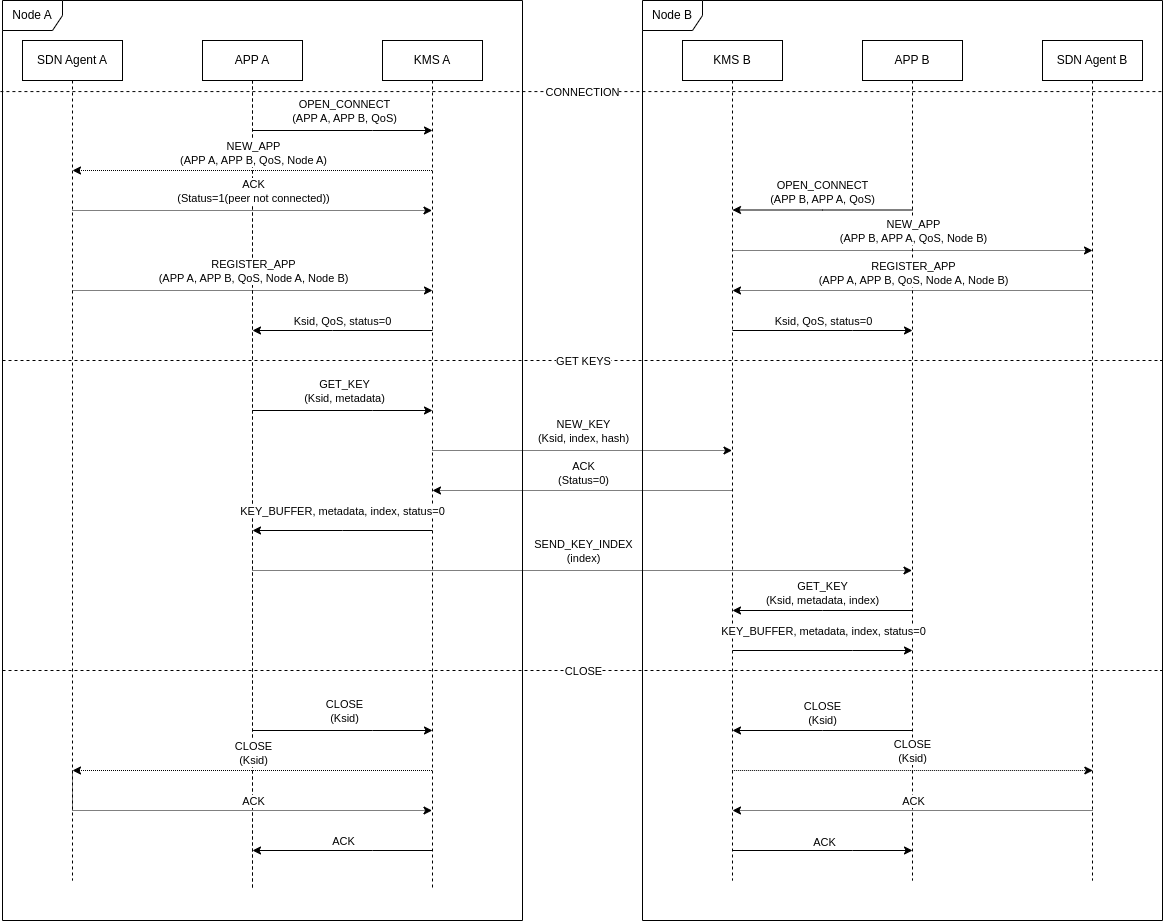
\includegraphics[width=15cm]{seq_diagram_0.png}
	\caption{Sequence diagram for a basic scenario with two directly connected nodes.}
	\label{fig:seq0}
\end{figure}

The workflow description associated with the sequence diagram (\autoref{fig:seq0}) is as follows:
\begin{itemize}
 	\item In node A, APP A makes an OPEN\_CONNECT request in order to create a connection to the \ac{KMS}. The goal of APP A is to communicate to APP B and vice-versa, so the \textit{source} is APP A, the \textit{destiny} is APP. 
 	\item \ac{KMS} A agrees on the QoS parameters proposed by the APP A. In order to know the location of APP B, sends a NEW\_APP request to the SDN Agent A.
 	\item In the instant that the SDN Controller is informed of the connection of APP A to KMS A in node A, APP B is to yet connected, so the SDN Agent acknowledges the NEW\_APP request  with a status code informing that the peer app is not connected.
 	\item In node B, APP B makes a OPEN\_CONNECT and the SDN Controller is notified via SDN Agent B.
 	\item With both applications connected the SDN Controller creates a global unique \textit{ksid} and, since Node A and Node B are directly connected, simply informs both \ac{KMS}s via the SDN Agents of the \textit{ksid} and \textit{qkdn\_id} of both nodes.
 	\item Both \ac{KMS} answer to the OPEN\_CONNECT request made previously by indicating the QoS and \textit{ksid} inherent to the connection.
 	\item App A makes a GET\_KEY request, giving the ksid and the metadata field only with the Metadata\_size that dictates the maximum size of the metadata buffer.
 	\item KMS A notifies KMS B of the creation of a new key for a specific \textit{ksid}. The \textit{index} field is not the index of the key to be created but the index of the raw key material from where the key will be extracted and it's optional. The \textit{hash} field is used for KMS B to check the integrity of the key that will be created. KMS B creates the key and acknowledges with a successful status code.
 	\item KMS A creates the key too and sends it to APP A alongside its metadata and index. The metadata might include creation and expiration timestamps and key type.
 	\item APP B receives a key index (how it's sent is out of the scope of the \ac{KMS}) and requests the key to \ac{KMS} B that responds with a key matching the one received previously by APP A. It's important to note that the result of this GET\_KEY request would be the same if no index would be provided by the application, since the oldest active key attached to this key stream is the one withe that index.
 	\item Both applications send a CLOSE request to their respective \ac{KMS}s to terminate the given key stream. The SDN Agents (consequently the SDN Controller too) are notified. Finally, both applications CLOSE request is acknowledge.
 	
\end{itemize}

\pagebreak

%%%%%%%%%%%%%%%%%%%%%%%%%%%%%%%%%%%%%%
% Acronyms
%%%%%%%%%%%%%%%%%%%%%%%%%%%%%%%%%%%%%%
\clearpage
\subsection*{Acronyms}\label{sec:acronyms}
\begin{acronym}[TDMA]
	\acro{KML}[KML]{Key Management Layer}
	\acro{KMS}[KMS]{Key Management System}
	\acro{KSID}[KSID]{Key Stream Id}
	\acro{SDN}[SDN]{Software Defined Network}
	\acro{RNG}[RNG]{Random Number Generator}
	\acro{DB}[DB]{Database}
	\acro{OTP}[OTP]{One Time Pad}
	\acro{ITS}[ITS]{Information-Theoretic Security}
	\acro{MAC}[MAC]{Message Authentication Code}
	\acro{KEM}[KEM]{Key Encapsulation Mechanism}
\end{acronym}
\pagebreak 


%%%%%%%%%%%%%%%%%%%%%%%%%%%%%%%%%%%%%%
% References
%%%%%%%%%%%%%%%%%%%%%%%%%%%%%%%%%%%%%%

% bibliographic references for the section 
\clearpage
\subsection{References}

\begin{enumerate}
	\item ETSI GS QKD 004, V2.1.1, 2020-08
	\item ETSI GS QKD 015, V2.1.1, 2022-04
	\item Discretion D3.1 SDN Preliminary Design Report, 2023
	\item ETSI GS QKD 014, V1.1.1, 2019-02
	\item Multiple stochastic paths scheme on partially-trusted relay quantum key distribution network, Hao, 2009
\end{enumerate}

\clearpage
\printbibliography[heading=subbibliography]
\end{refsection}
\addcontentsline{toc}{subsection}{Bibliography}
\cleardoublepage
 
\clearpage\clearpage
\graphicspath{{sdf/key_management_layer/figures/}}
\acresetall


\section{ETSI QKD 004}
\label{etsi_004}
% Show subsubsections on the Table of Contents
\setcounter{tocdepth}{3}
\setcounter{secnumdepth}{3}

\begin{refsection}
	\begin{tcolorbox}
		\begin{tabular}{p{2.75cm} p{0.2cm} p{10.5cm}}
			\textbf{Goal}          &:& Implementation of the ETSI GS QKD 004\\
			\textbf{Directory}     &:& sdf/dv\_qkd\_ldpc\\
			\textbf{Contributors}   &:& Armando Nolasco Pinto (2021/01/22 - ) \\
									&& Diogo Silva (2021/03/29 - ) \\
		\end{tabular}
	\end{tcolorbox}



\subsection{Introduction}

The security of cryptographic keys negotiated through an insecure communication channel is only ensured by the amount of computational power required to break it, to the point where it becomes unpractical to try to break them. 
This is done with using one-way functions. One-way functions are functions where it is easy to compute its output given a certain input but it is hard to do the reverse process. This makes it so that if someone eavesdrop the key negotiation channel and wants to get the negotiated key they have to test every possibility until they find a match. So if the keys are big enough they are considered secure, although the security of these keys is only assured by the difficulty of the reverse process, which is not mathematically proven. Usually the security of the keys is increased by making them bigger. However, with the presence of quantum computers, these methods become insecure. This is due to quantum computers being very fast at factoring large numbers. Because of this there is a need to create cryptographic key negotiation methods which do not become obsolete in the presence of quantum computers. ETSI Quantum Key Distribution protocol is a method for negotiating cryptographic keys whose security is ensured by the laws of physics, so they cannot be broken either by classic computers or quantum computers. These keys will be negotiated through a quantum channel controlled by specific equipment. The keys can then be distributed to applications via a key management layer which communicates directly with the QKD system. This key management layer is defined in the ETSI QKD 004 standard. 

\subsection{Key Management Layer}

Although the QKD system manages the exchange of cryptographic keys, those keys need to be distributed and synced with the various applications that will use them. This is done by the Key Management Layer. This layer will ensure that the applications that communicate with each other at both ends use the same cryptographic key. The Key Management Layer provides the applications with an API (Application Programming Interface) for them to interact with the QKD System. The interface must have the following functions: 

\begin{lstlisting}
	OPEN_CONNECT(in source, in destination, inout QoS, inout Key_stream_ID, out status)
	GET_KEY(in Key_stream_ID, inout index, out Key_buffer, inout Metadata, out status)
	CLOSE(in Key_stream_ID, out status)
\end{lstlisting}

\pagebreak

\begin{itemize}
	
	\item\underline{OPEN\textunderscore CONNECT(in source, in destination, inout QoS, inout Key\textunderscore stream\textunderscore ID, out status)}
	
		This function associates a Key\textunderscore stream\textunderscore ID to a set of future keys at both ends of the QKD system and establishes a set of parameters for the key service specified by the QoS structure. This function blocks until the peers are connected or the Timeout value is exceeded.
	
	\item\underline{GET\textunderscore KEY(in Key\textunderscore stream\textunderscore ID, inout index, out Key\textunderscore buffer, inout Metadata, out status)}
	
		This function returns the required amount of key material requested for this specific Key\textunderscore stream\textunderscore ID. In case it does not return the key material it should return a error message. The QKD Management Layer should return an index value for the specified key. This index is used for synchronization purposes. The key position will be the result of multiplying the index value by the Key\textunderscore chunk\textunderscore size value. 
		
	\item\underline{CLOSE(in Key\textunderscore stream\textunderscore ID, out status)}
	
		This function verifies if the QKD link is available and the key\textunderscore handle association is synchronized at both ends of the link. This function does not block and thus returns immediately indicating if both sides of the link are synchronized or if an error has occurred.
			
\end{itemize}

\subsubsection{Parameters}

The parameters used by the API functions are the following:

\begin{lstlisting}
	Key_stream_ID
	Key_buffer
	Index
	Source
	Destination
	QoS
	Metadata
	Status
\end{lstlisting}

\begin{itemize}
	
	\item\underline{Key\textunderscore stream\textunderscore ID}
		
		The Key\textunderscore stream\textunderscore ID is a unique identifierfor the group of bits provided by the QKD Key Manager to the application. It is a 16 bytes UUID (Universally unique identifier).
	
	\item\underline{Key\textunderscore buffer}
	
		The key\textunderscore buffer is a buffer containing the current stream of keys. It should be stored as an array of bytes.
		
	\item\underline{Index}
	
		Position of the key to be accessed within the reserved key store for the application. Should be stored as a 32 bit unsigned integer
		
	\item\underline{Source}
	
		Identifier of the source application connection to the QKD key management layer. The identifier is structured as an URI.
		
	\item\underline{Destination}
	
		Identifier of the destination application connecting to the QKD key management layer. The identifier is structured as an URI.
		
	\item\underline{QoS}
	
		The QoS parameters is a structure composed by the following parameters:
		
		\begin{itemize}
			\item{Key\textunderscore chunk\textunderscore size}
				
				Length of the key buffer requested by the application. 32 bit unsigned integer.
				
			\item{Max\textunderscore bps}
			
				Maximum key rate requested in bits per seconds. 32 bit unsigned integer.
				
			\item{Min\textunderscore bps}
			
				Minimum key rate requested in bits per seconds. 32 bit unsigned integer.
				
			\item{Jitter}
				
				Maximum expected deviation, in bps, for key delivery. 32 bit unsigned integer.
				
			\item{TTL (Time to Live)}
			
				Time after which the keys corresponding to this Key\textunderscore stream\textunderscore ID shall be erased. 32 bit unsigned integer.
				
			\item{Metadata mimetype}
			
				Field that defines the format of the metadata on each subsequent GET\textunderscore KEY call. Char array of size 256.
				
		\end{itemize}
	
	\item\underline{Metadata}
		
		\begin{itemize}
			\item{Metadata\textunderscore size}
				Size of metadata buffer in characters. 32 bit unsigned integer.
				
			\item{Metadata\textunderscore buffer}
				Buffer for the returned metadata.

		\end{itemize}
		
	\item\underline{status}
	
		32 bit unsigned integer that indicates the success or failure of the request. The output values are the following:
		
		\begin{itemize}
			\item{0: }
				Successful
			\item{1: }
				Successful connection, but peer not connected.
			\item{2: }
				QKD\textunderscore GET\textunderscore KEY failed because insufficient key available.
			\item{3: }
				QKD\textunderscore GET\textunderscore KEY failed because peer application is not yet connected.
			\item{4: }
				No QKD connection available.
			\item{5: }
				OPEN\textunderscore CONNECT failed because the Key\textunderscore stream\textunderscore ID is already in use.
			\item{6: }
				TIMEOUT\textunderscore ERROR. The timeout has been exceeded.
			\item{7: }
				OPEN failed because requested QoS settings could not be met, counter proposal included in return has occurred.
			\item{8: }
				GET\textunderscore KEY failed because metadata field size insufficient. Returned Metadata\textunderscore size value holds minimum needed size of metadata.
		\end{itemize}
			
\end{itemize}

\subsubsection{Notes}

Some additional considerations to be taken into account are:
\begin{itemize}
	\item
		An application may request various different keys and there is no limit to the number of key streams a given application can request. The only requirement is that the Key\textunderscore stream\textunderscore ID must be different. 
	\item
		The Key\textunderscore stream\textunderscore ID must uniquely identify the key material and the key material cannot be derived from it.
	\item
		The Key\textunderscore stream\textunderscore ID may or may not be provided by the application. In case the application does not provide a Key\textunderscore stream\textunderscore ID the Key Management Layer should generate one and return it to the application.
\end{itemize}

\subsection{Extending QKD to oblivious keys}

ETSIs QKD protocol could be extended to use oblivious keys instead. For that we need to add API calls that deal with QOKD instead of QKD.

\begin{lstlisting}
	QOKD_OPEN_CONNECT(in source, in destination, inout QoS, inout Key_stream_ID, out status)
	QOKD_GET_KEY(in Key_stream_ID, inout index, out Key_buffer, inout Metadata, out status)
	QOKD_CLOSE(in Key_stream_ID, out status)
\end{lstlisting}

There is also a additional parameter needed, \texttt{role} , that serves the purpose of indicating if the application will play the role of Alice or Bob in the oblivious transfer because both parties follow different routines in the transfer and the Key Manager needs that information. 
The status parameter may return an additional error, \texttt{1024}, that indicates conflicting roles, in case both APPA and APPB try to play the same role in the OT.

\subsection{Use Case Examples}

\begin{itemize}
	\item
	APPA: Application at host A
	\item
	APPB: Application at host B
	\item
	KMA: QKD key manager at host A
	\item
	KMB: QKD key manager at host B
	\item
	QKSA: QKD system at host A
	\item
	QKSB: QKD system at host B
\end{itemize}

\subsubsection{QKD with undefined key\textunderscore handle}

\begin{figure}[H]
	\centering
	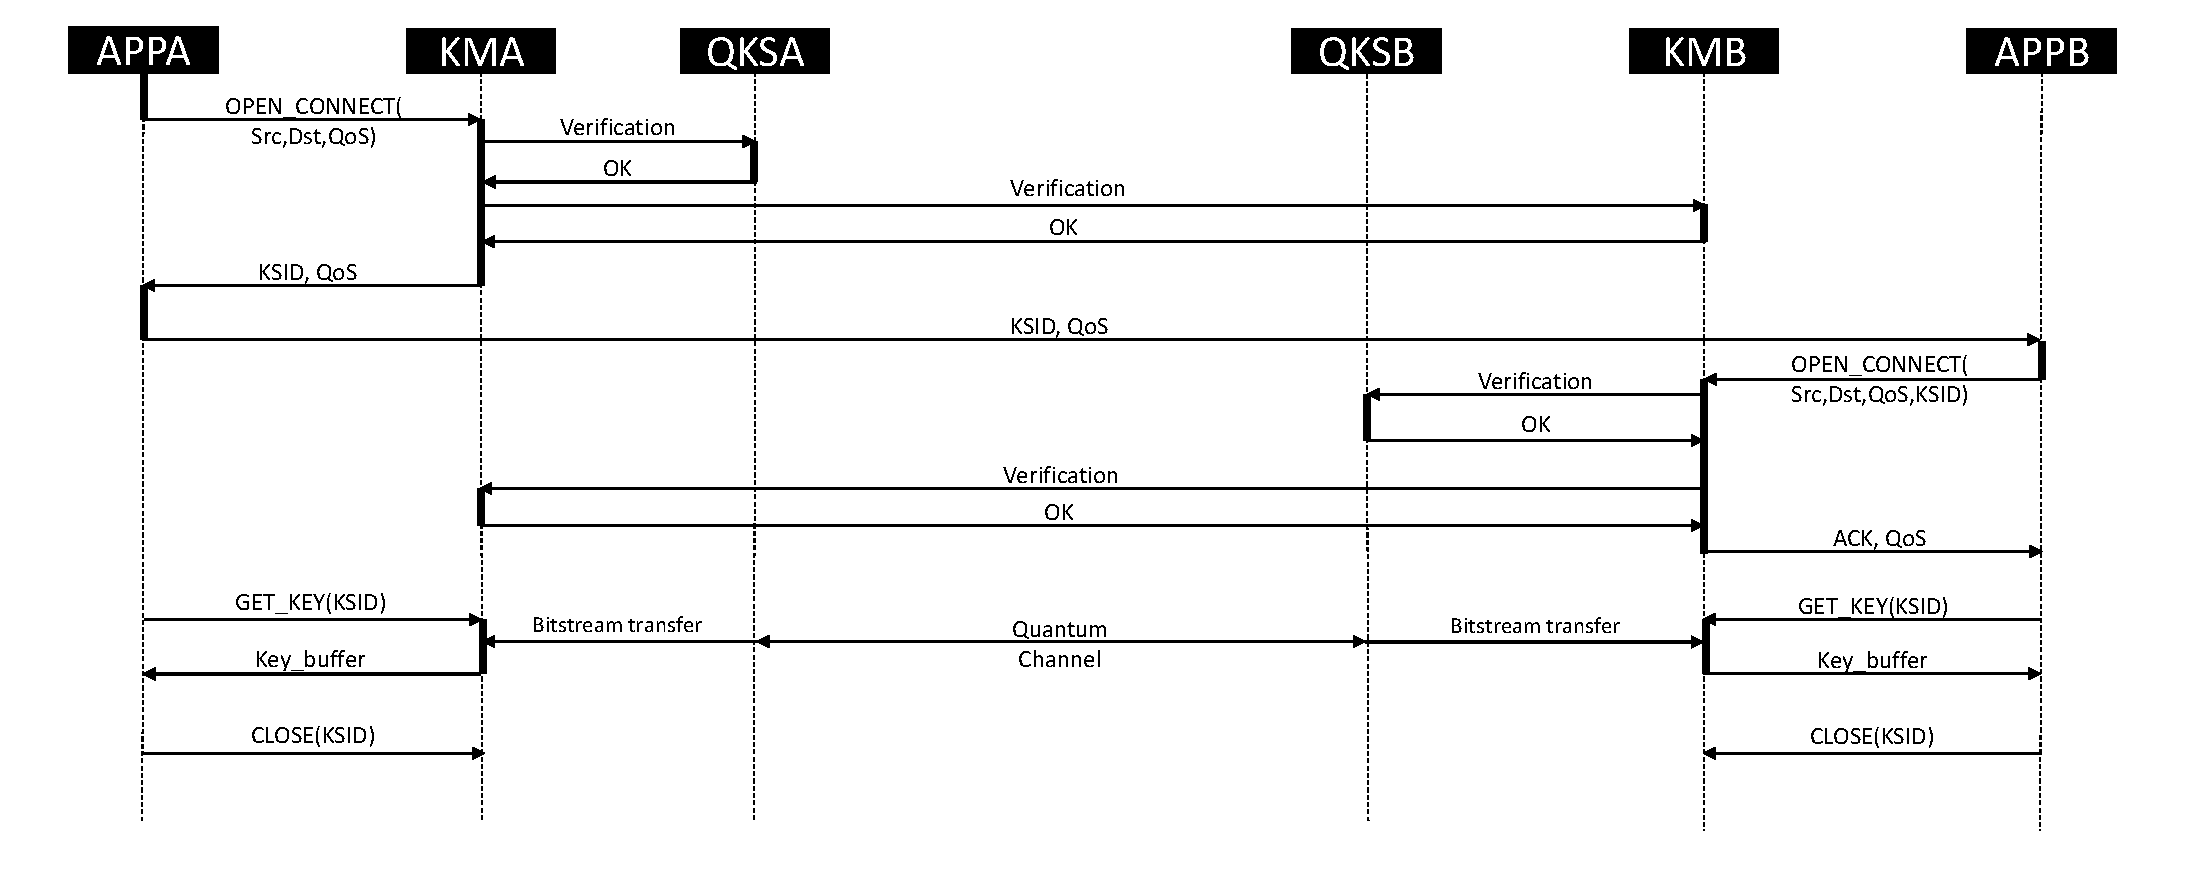
\includegraphics[width=15cm]{qkdUpdated.pdf}
	\caption{QKD with undefined Key\textunderscore stream\textunderscore ID}
	\label{fig:QKDUndefinedKSID}
\end{figure}

In this example APPA does not provide a Key\textunderscore stream\textunderscore ID. Because of that the Key Manager returns a generated Key\textunderscore stream\textunderscore ID, which the application has to send to the APPB to make sure that the KSID is synchronized at both ends.

\subsection{Block Diagram}

%\begin{figure}[H]
%	\centering
%	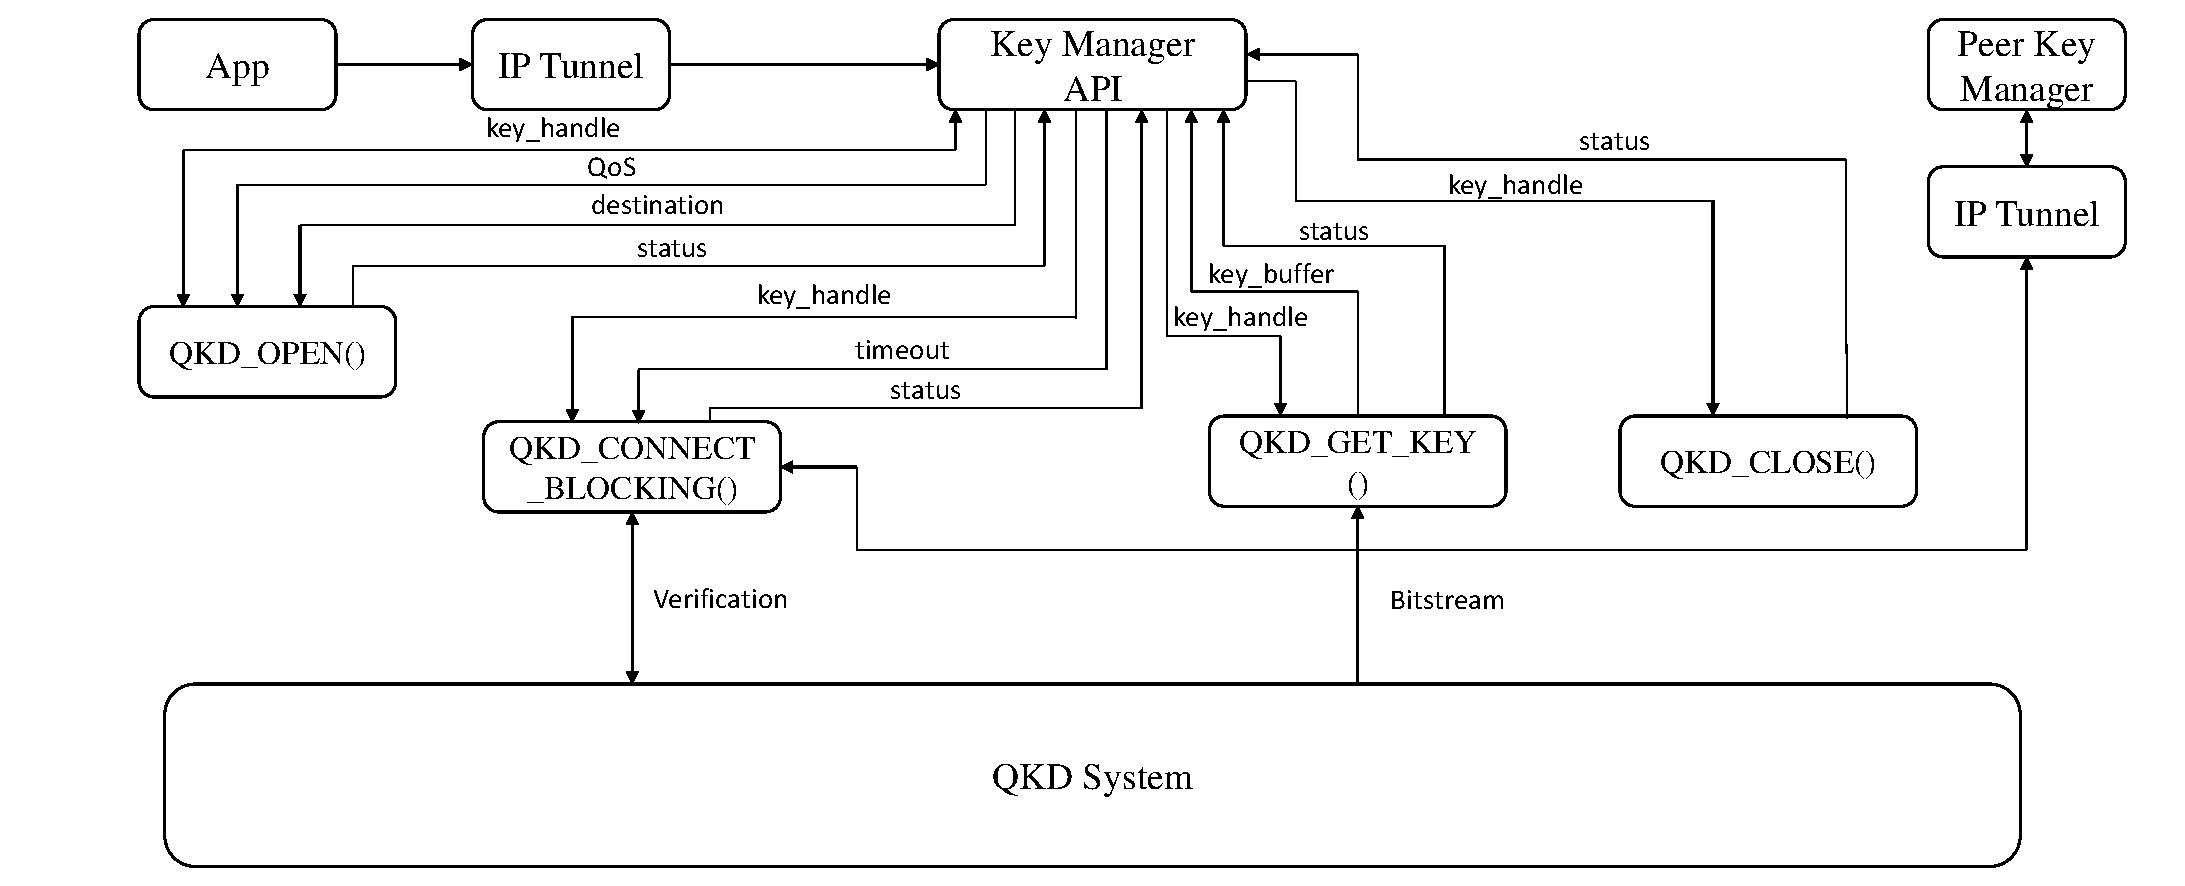
\includegraphics[width=15cm]{blockDiagram.pdf}
%	\caption{Block Diagram}
%	\label{fig:blockDiagram}
%\end{figure}

%\begin{figure}[H]
%	\centering
%	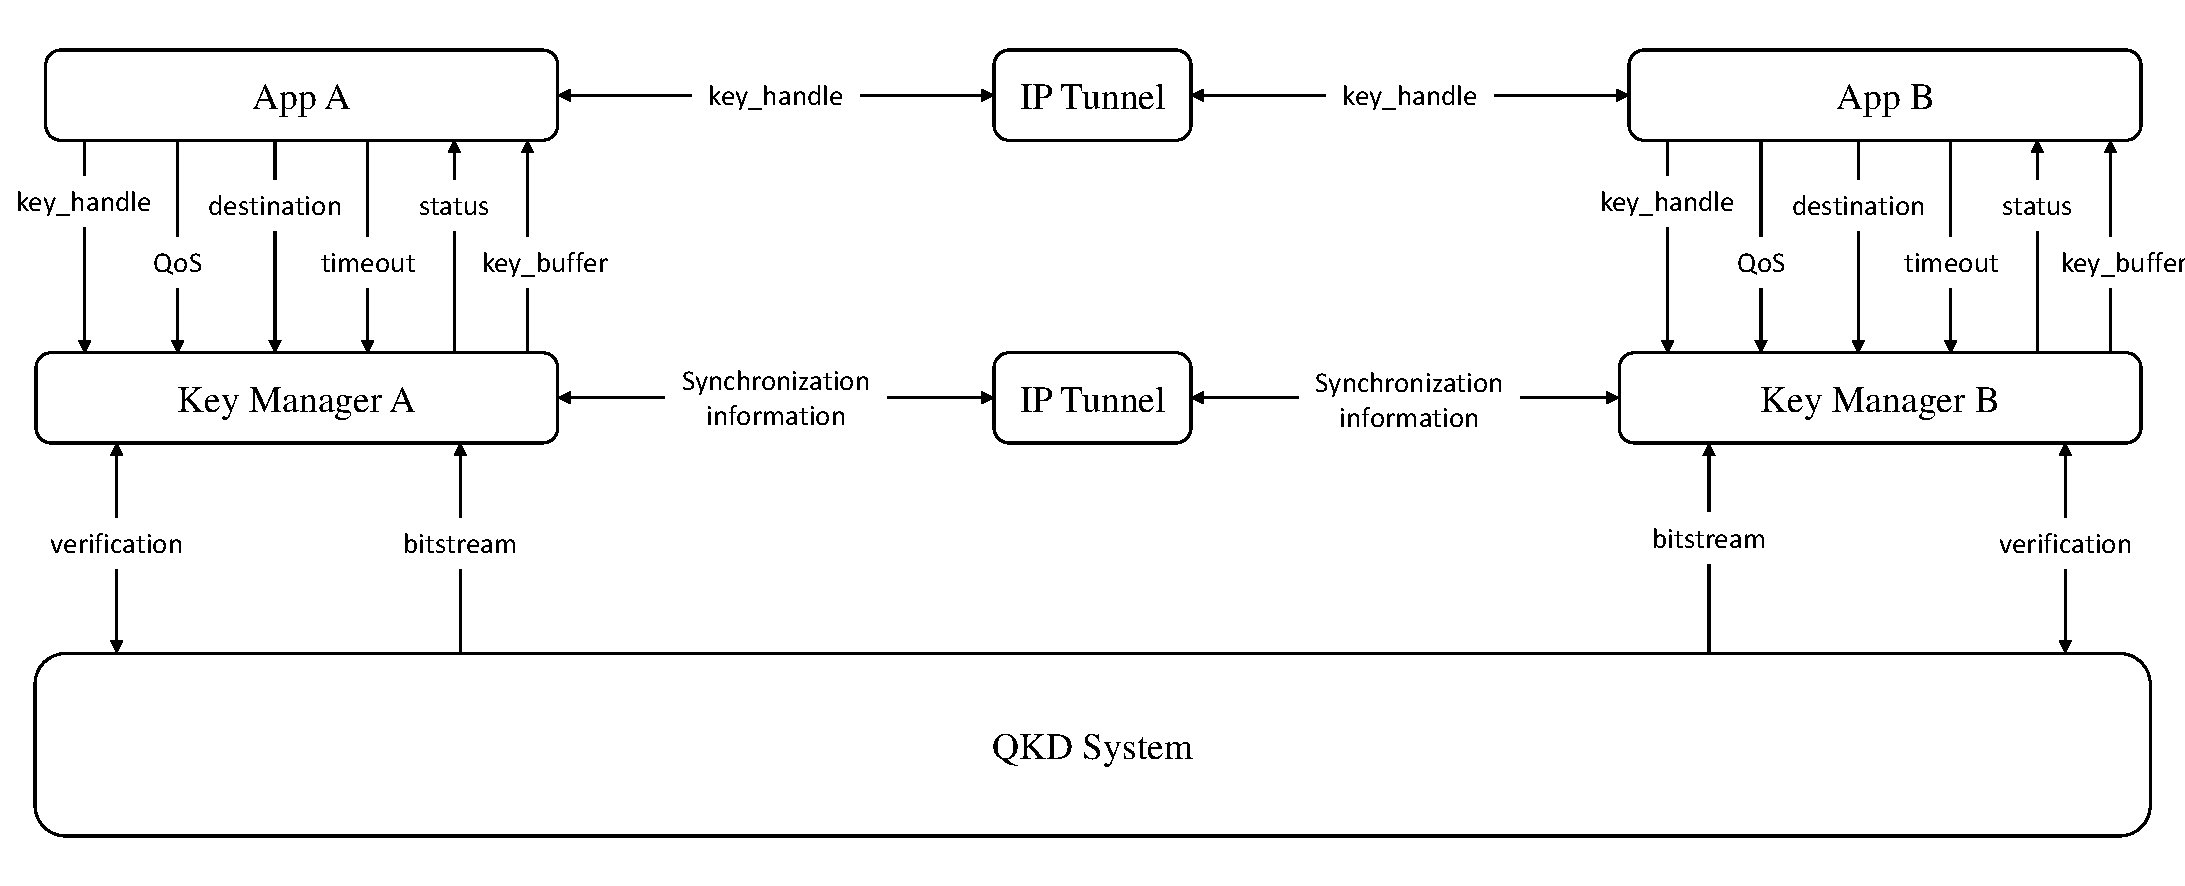
\includegraphics[width=15cm]{blockDiagram2.pdf}
%	\caption{Block Diagram 2}
%	\label{fig:blockDiagram2}
%\end{figure}

\begin{figure}[H]
	\centering
	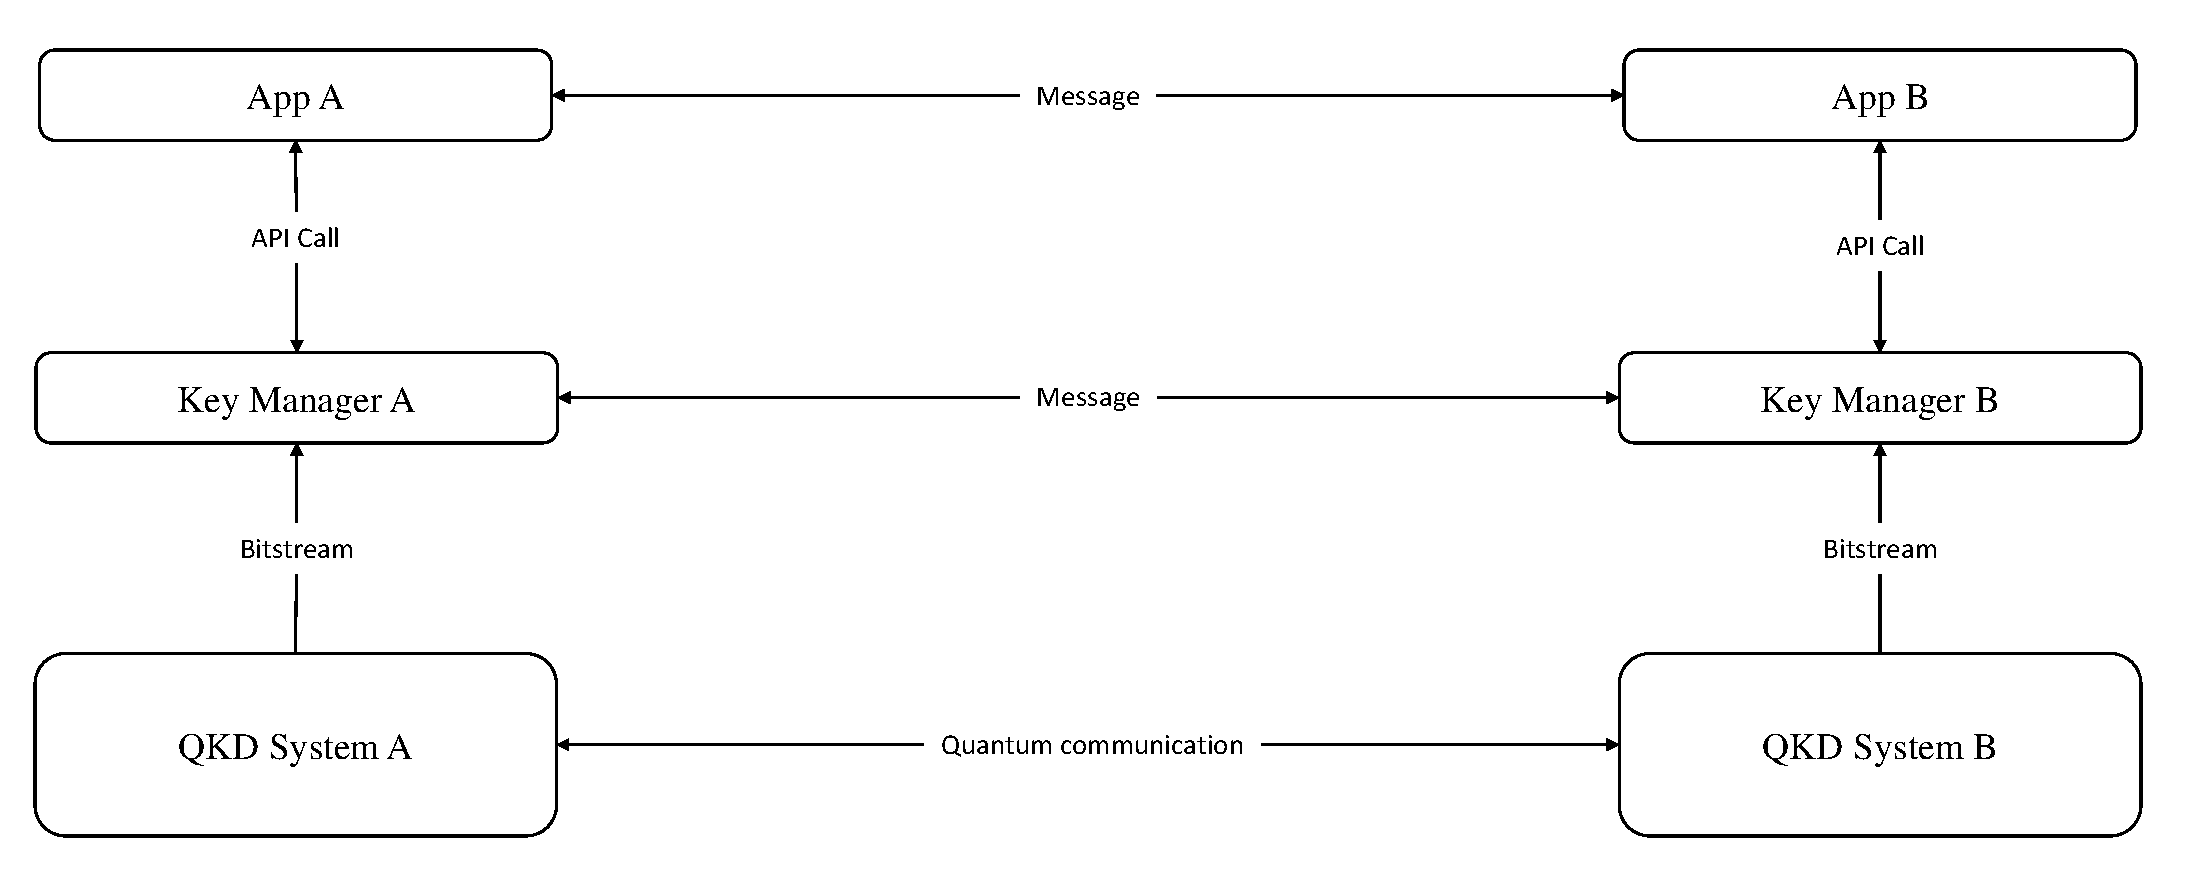
\includegraphics[width=15cm]{communicationsBlockDiagram.pdf}
	\caption{Communications Block Diagram}
	\label{fig:blockDiagram3}
\end{figure}

The objective of this system is to provide the same symmetric and oblivious keys to both applications (APP A and APP B). These keys will come from the QKD systems. The Key Management Layer is responsible to get the keys from the physical QKD system. From there there is a need for the Key Manager to communicate with its peer Key Manager for key synchronization purposes. The way this is done is left to the implementer. One simple example is a socket communication. From there both Apps need to get the keys from their respective Key Manager. This should be done through calls to an API. The technology used for this API is left to the implementer. Two examples of ways to implement this API are REST and a socket. The only requirement is that the API accepts data in json format. The communication between both Apps is left to the implementer. This need for this communication is to make sure that both Apps have the same Key\textunderscore stream\textunderscore ID.

\begin{figure}[H]
	\centering
	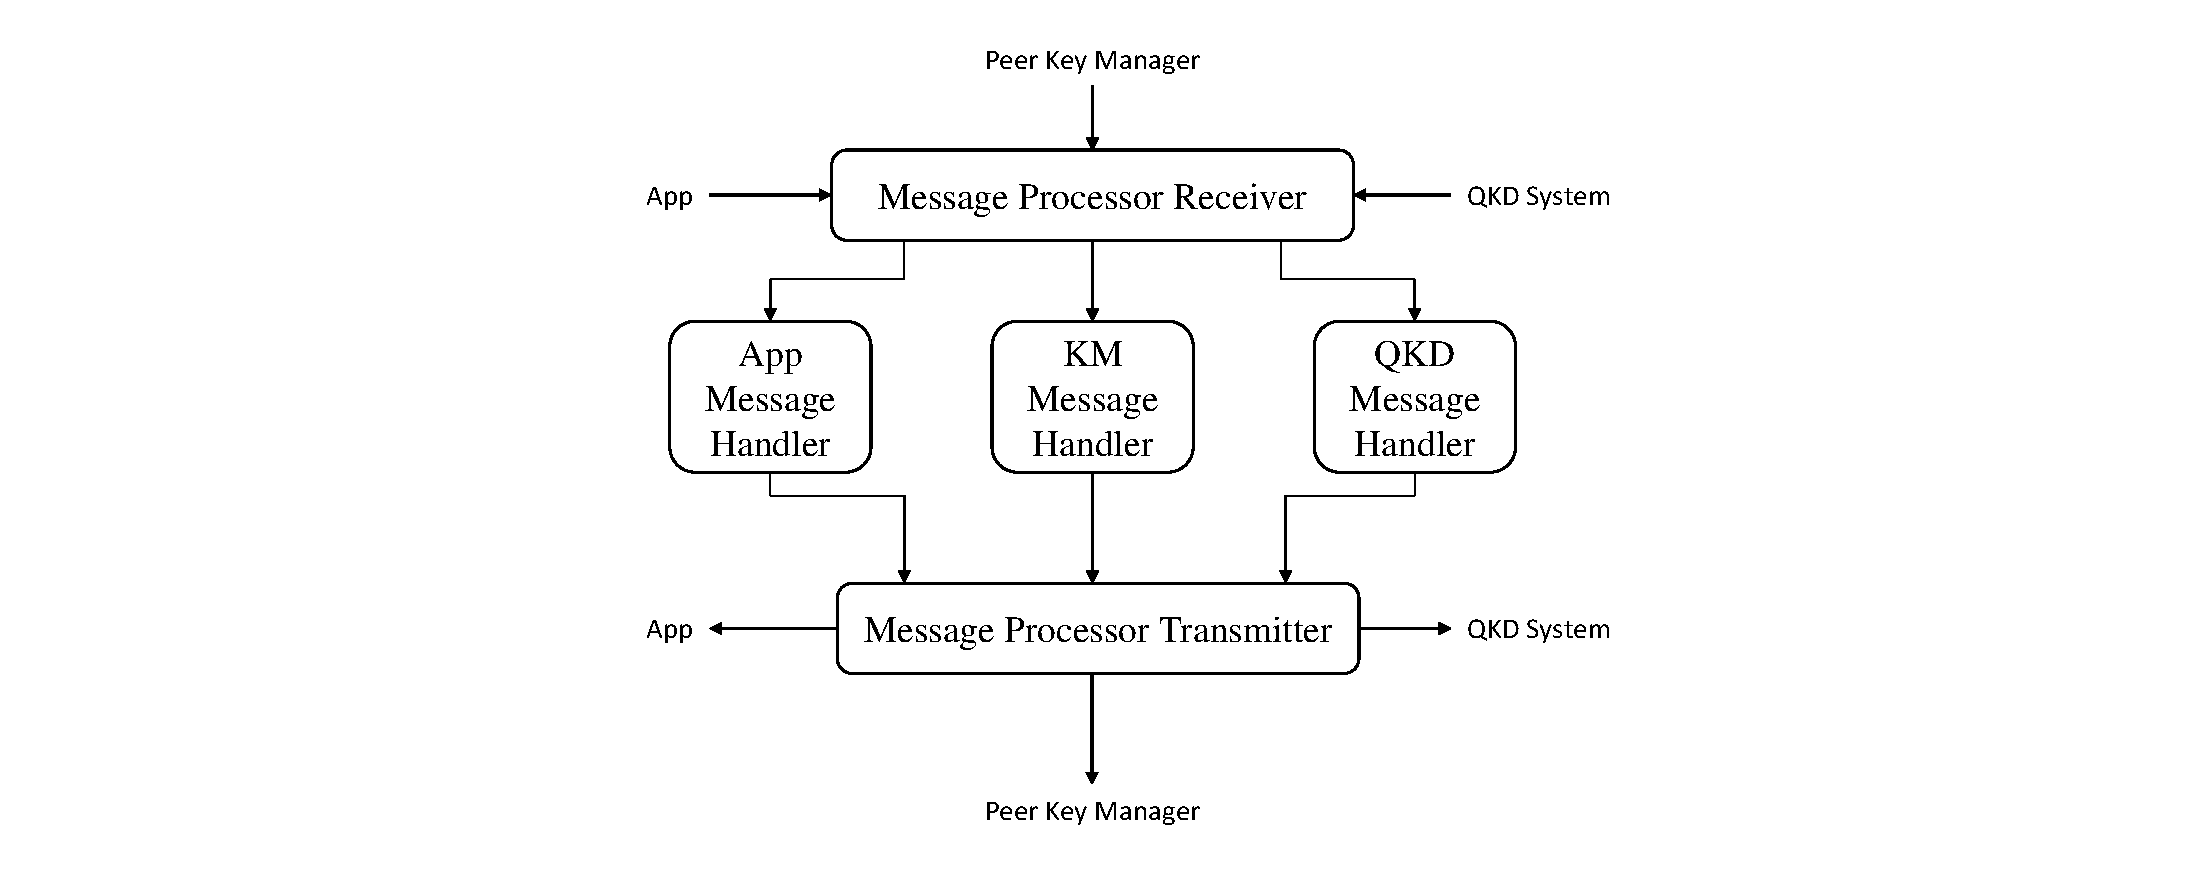
\includegraphics[width=15cm]{messageProcessor.pdf}
	\caption{Message Processor}
	\label{fig:blockDiagram4}
\end{figure}

Above is a simple diagram that illustrates the message processor of each Key Manager. The Receiver gets its input from the App, the Peer Key Manager and the QKD System. These inputs might come in different formats. The receiver than relays that information to the appropriate message handler, depending on who the input came from. Once the handlers have processed the information and return an answer, that information is send to the Message Processor Transmitter, whose job is to then send the response to the adequate system.

\subsection{Madrid Example}

A example was provided from our partners in Madrid. This example is written in Python 3.6. It is a generic 004 implementation that has no hardware connection to the QKD system, and so it simulates it by generating a random key. There is a script that simulates two applications exchanging messages encrypted with the keys provided by the LKMS. The LMKS's can be run without the applications and used with our own application.

\subsection{Socket Description}

\begin{figure}[H]
	\centering
	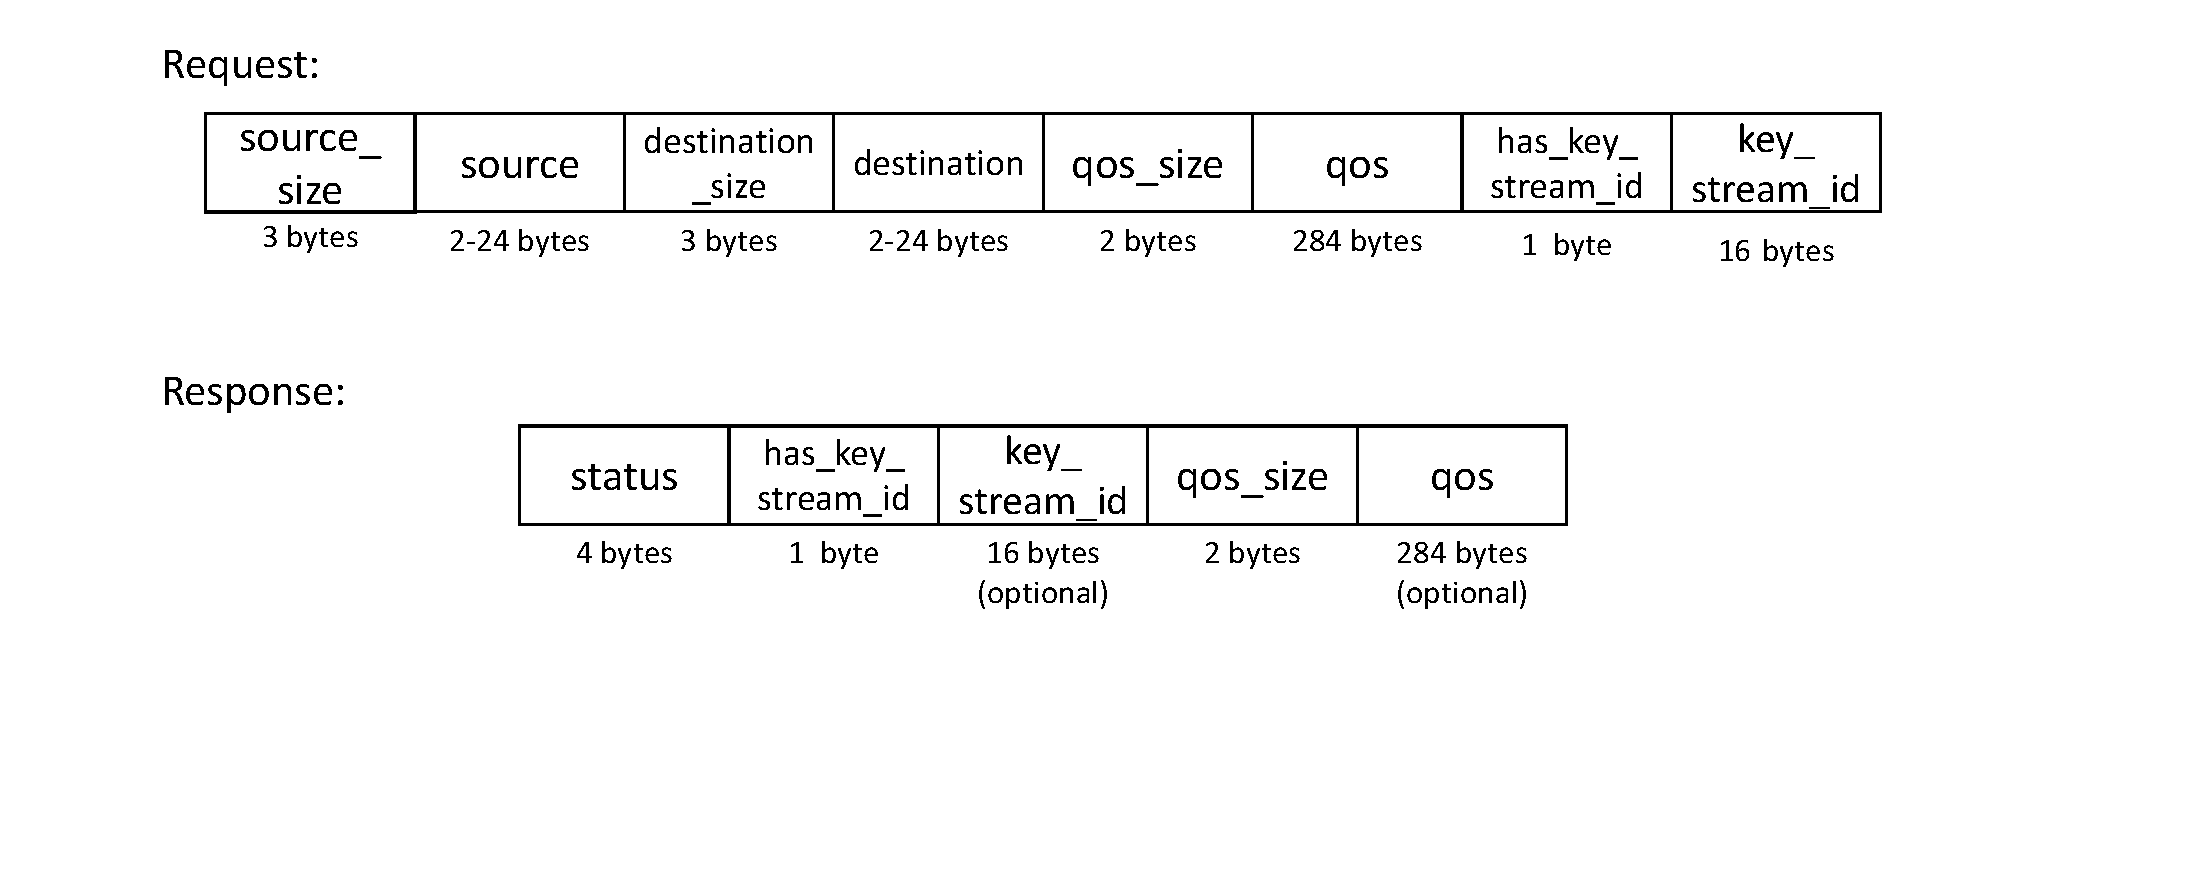
\includegraphics[width=15cm]{open_connect_socket.pdf}
	\caption{Open Connect Socket}
	\label{fig:openConn}
\end{figure}

\begin{itemize}
	\item\underline{source}
		
		URI of the source

	\item\underline{source\textunderscore size}

		Size of the source URI

	\item\underline{destination}

		URI of the destination

	\item\underline{destination\textunderscore size}

		Size of the destination URI

	\item\underline{qos\textunderscore size}

		Size of the QoS structure

	\item\underline{qos}

		QoS structure

	\item\underline{has\textunderscore key\textunderscore stream\textunderscore id}

		Informs if the request provides a KSID

	\item\underline{key\textunderscore stream\textunderscore id}

		KSID provided by the application (optional)

	\item\underline{status}

		Status code returned by the KMS

\end{itemize}

\begin{figure}[H]
	\centering
	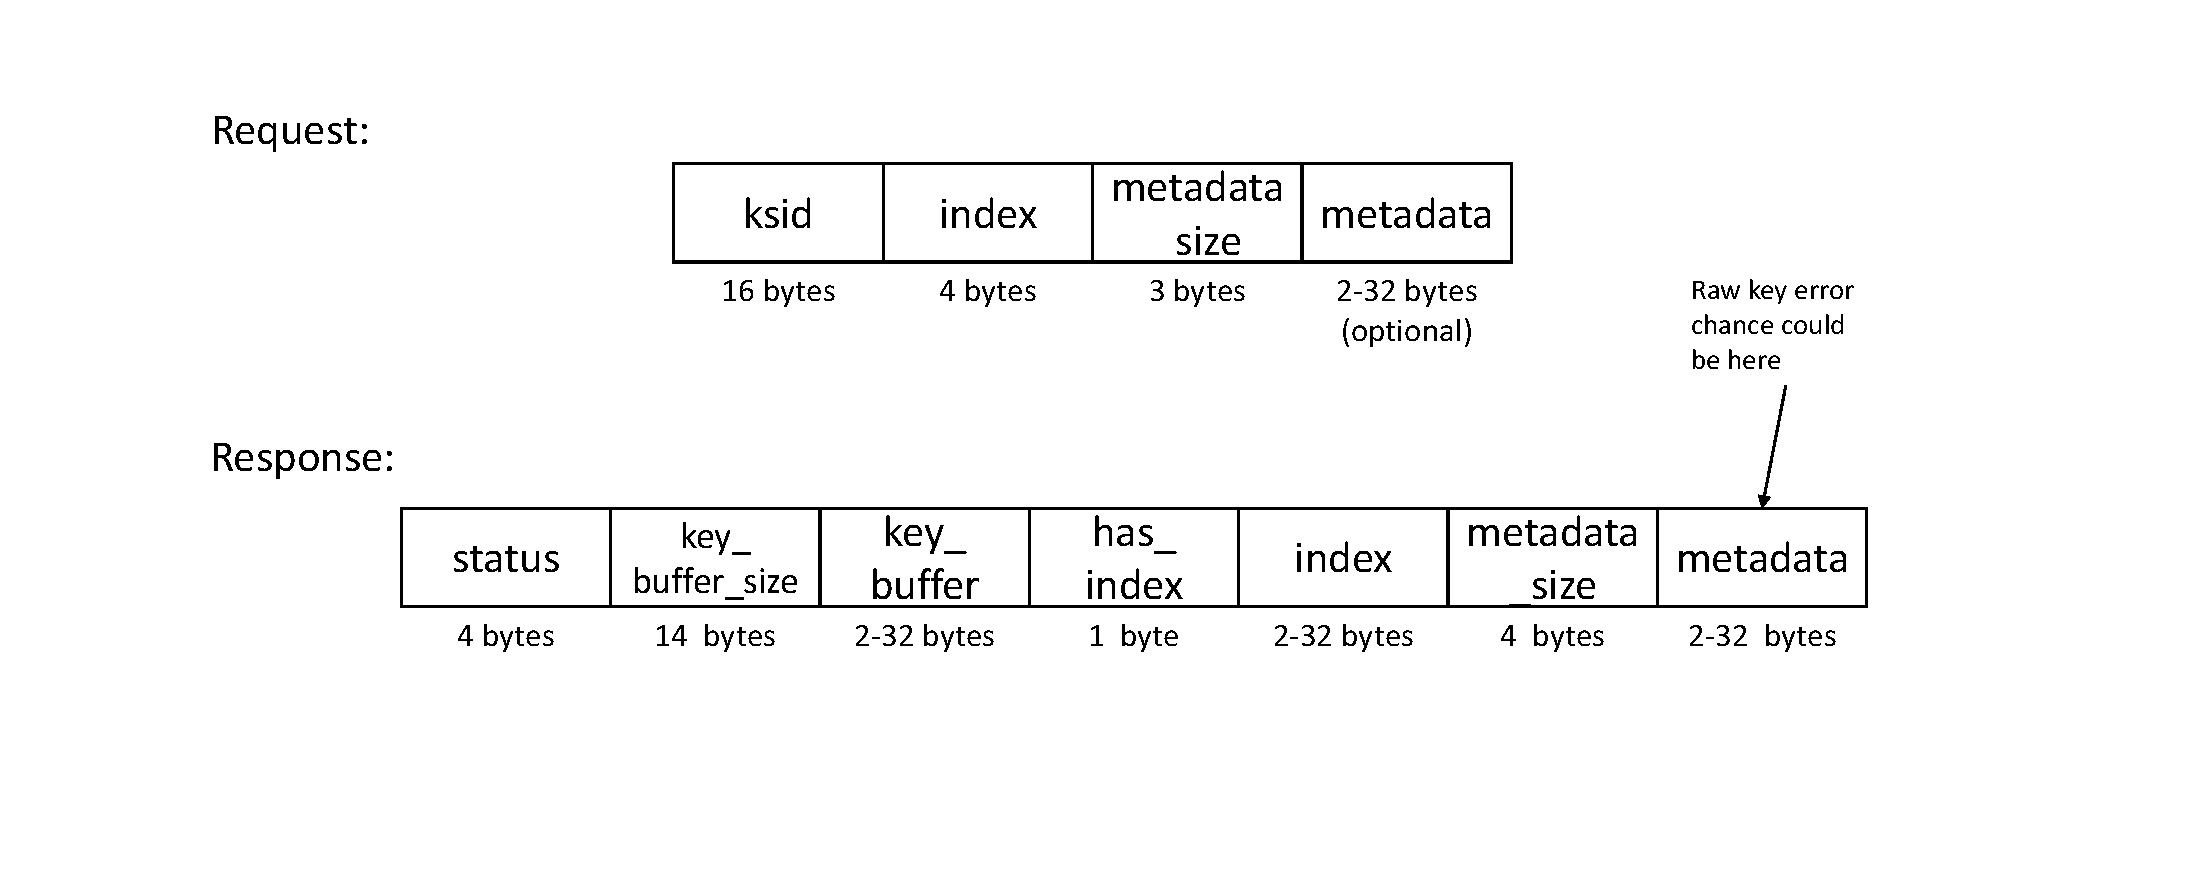
\includegraphics[width=15cm]{get_key_socket.pdf}
	\caption{Get Key Socket}
	\label{fig:getKey}
\end{figure}

\begin{itemize}

	\item\underline{ksid}

		KSID

	\item\underline{index}

		Position of the key to be accessed within the reserved key store for the application

	\item\underline{metadata\textunderscore size}

		Size of the metadata parameter

	\item\underline{metadata}

		Metadata about the key requested/provided

	\item\underline{status}

		Status code returned by the KMS

	\item\underline{key\textunderscore buffer\textunderscore size}

		Size of the key buffer

	\item\underline{key\textunderscore buffer}

		Key Buffer

	\item\underline{has\textunderscore index}

		Field that indicates if the key index is provided

\end{itemize}

\begin{figure}[H]
	\centering
	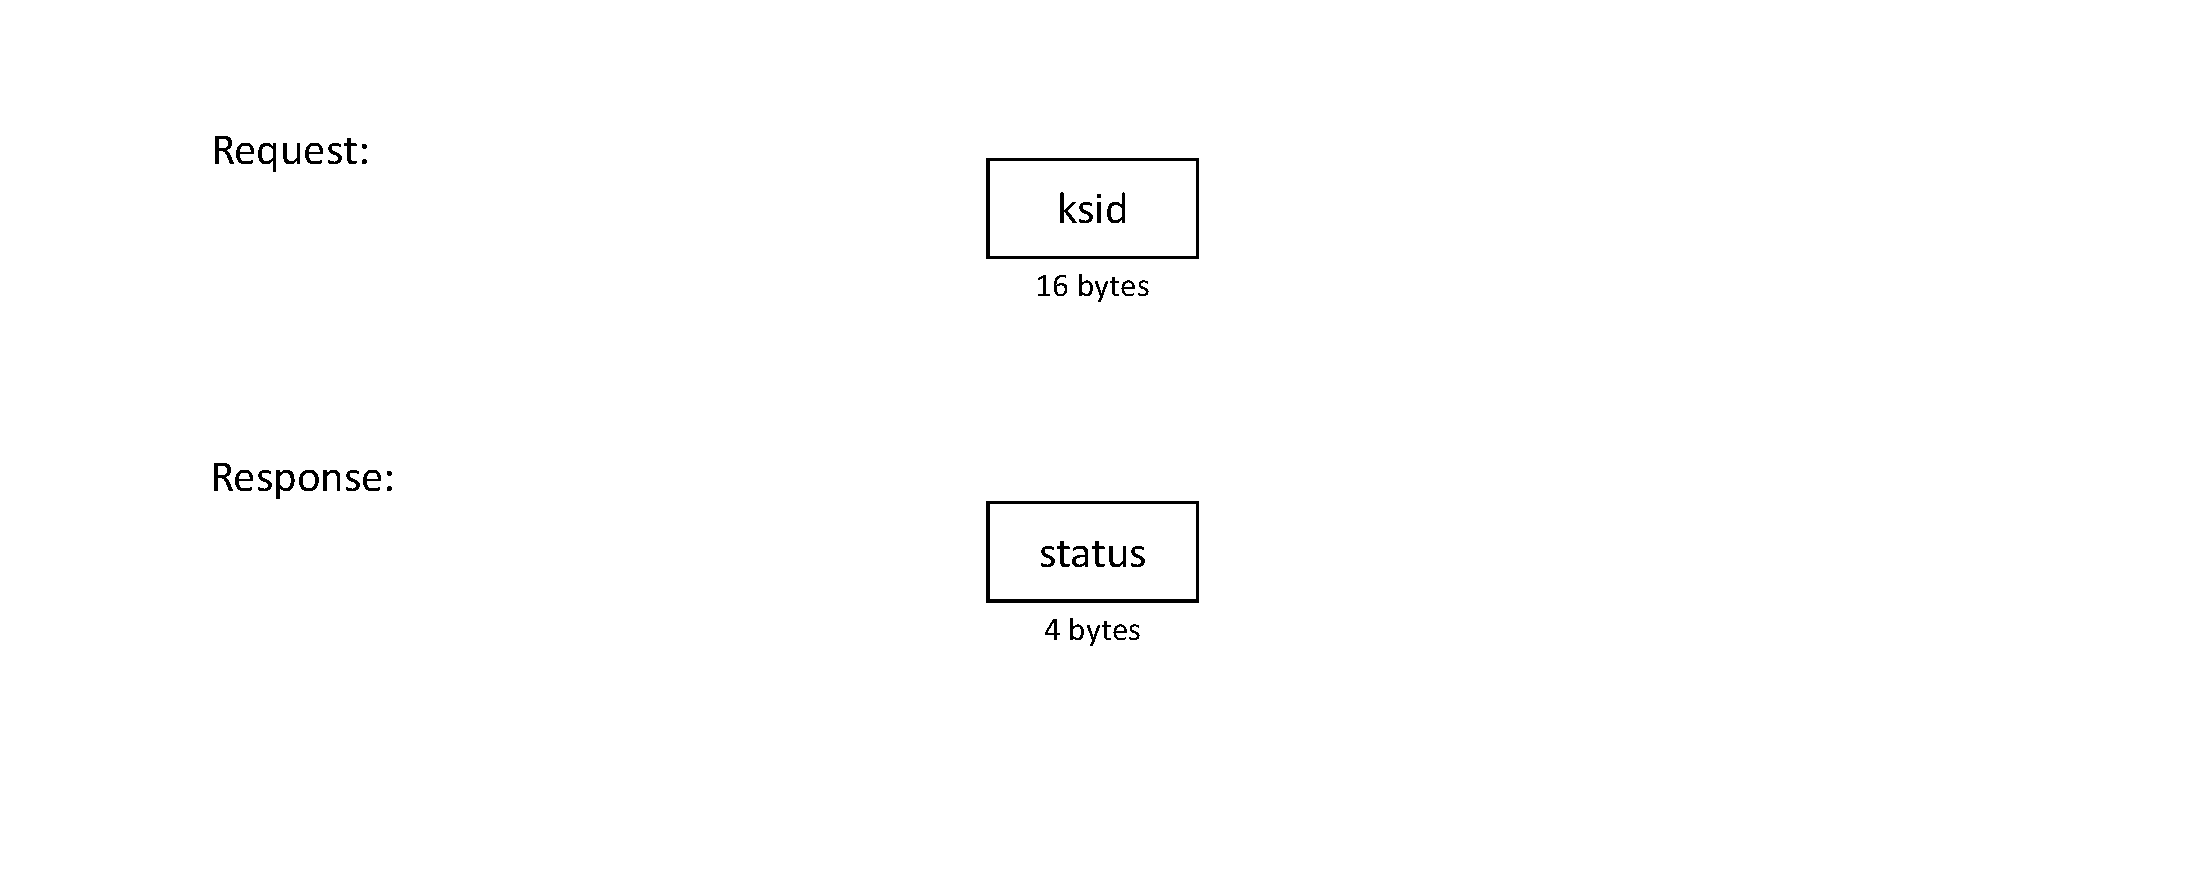
\includegraphics[width=15cm]{close_socket.pdf}
	\caption{Close Socket}
	\label{fig:close}
\end{figure}

\begin{itemize}

	\item\underline{ksid}

		KSID

	\item\underline{status}

		Status code returned by the KMS

\end{itemize}

\subsubsection{Setting up the virtual environment and dependencies}

Before running the example we need to make sure we are using a virtual environment (to have a clean installation), the right python version and the its dependencies.
The first step is to install python 3.6 and gcc, running the following command:

\texttt{sudo apt install -y python3.6-dev gcc virtualenv}

To make sure the right version of python is installed we can run python3 with the --version argument: 

\texttt{python3 --version}

Having python 3.6 installed we can proceed. The next step is to head over to the example directory, \texttt{sdf/etsi\textunderscore qkd\textunderscore 004/madrid\textunderscore example/} and open a terminal there so we can make a virtual environment. To install the virtual environment simply run the command:

\texttt{virtualenv -p python3 qkd004}

This will create a virtual environment with the name \texttt{qkd004}. After installing it we need to activate it. Run the command:

\texttt{source qkd004/bin/activate}

Upon the virtual environment we can install the needed python dependencies by running the command:

\texttt{pip install -r requirements.txt}

At this point, provided there were no errors, everything should be set for running the example.

The scripts should be used inside the virtual environment. After using it, to leave the virtual environment, simply type the command:

\texttt{deactivate}

\subsection{Running the example}

Two run the example simply run the command:

\texttt{python run\textunderscore test.py}

This example will spawn two LKMS and two applications using threads. These applications will exchange messages encrypted with symmetric keys provided by the LMKS.

\begin{figure}[H]
	\centering
	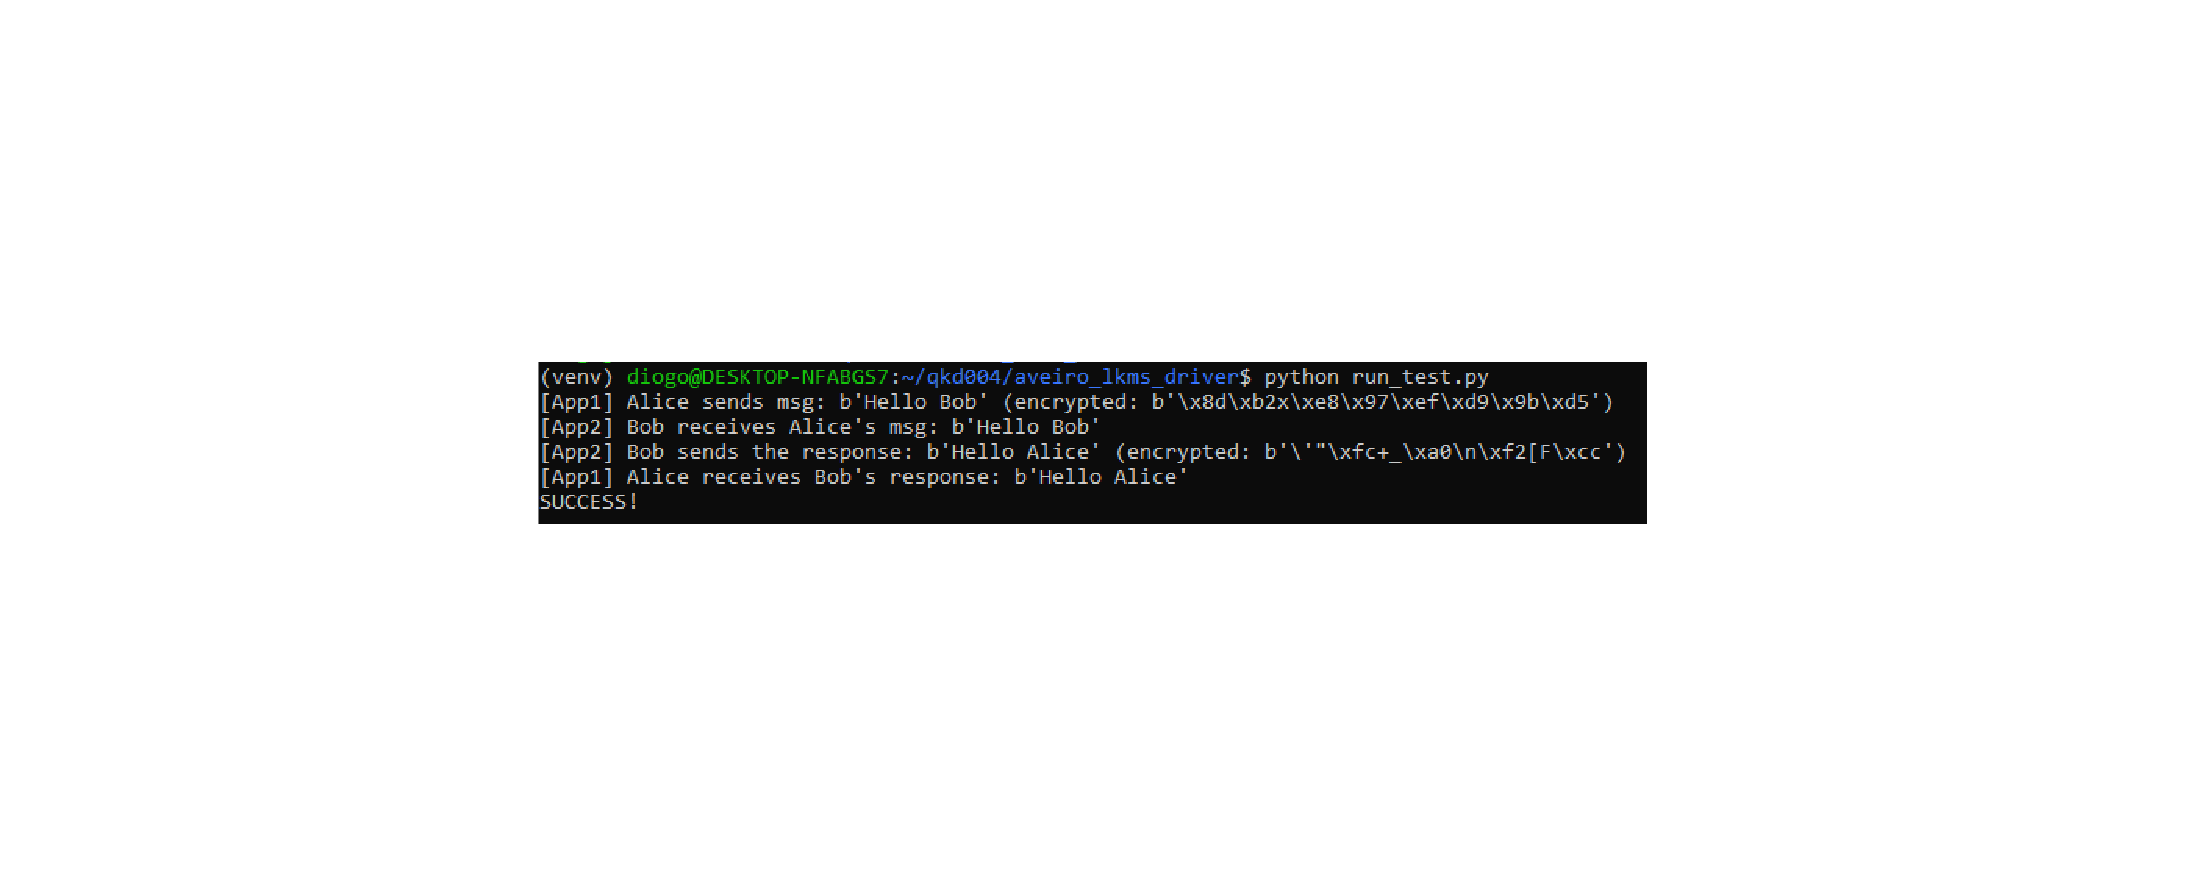
\includegraphics[width=15cm]{madridExample.pdf}
	\caption{Madrid Example}
	\label{fig:madridExample}
\end{figure}

\subsection{Running only two LKMS}

To run the LKMS without running the applications we must first install the qkd004 implementation as a python module by running the following command:

\texttt{pip install etsi\textunderscore qkd\textunderscore 004/}

After that simply run the script \texttt{run\textunderscore lkms.py}:

\texttt{python run\textunderscore lkms.py}

This will spawn two LMKS on separate threads, one in port 44441 and another in port 44442, both on localhost. To change the port or address simply edit lines 5 and 6 of the script.

\subsection{Using the Application driver}

The Madrid example includes a driver for the application. This driver includes functions that implement the socket communication needed to interact with the LMKS API. To use this driver you also need to install the etsi\textunderscore qkd\textunderscore 004 module as described above. Note that you should import the driver at the start of the python script with the following line:

\texttt{from aveiro\textunderscore driver.app\textunderscore 004 import *}

This driver really simplifies the application implementation as there is only the need to initialize the application driver object. From then on if there is the need to encrypt messages just use the encrypt and decrypt method of the application driver.

First declare the variables needed (lkms address, source URI, destination URI and QoS):

\texttt{lkms\textunderscore node1\textunderscore address = ("localhost", 44441)}

\texttt{source = URI("qkd://Application1@aaaaaaaa-aaaa-aaaa-aaaa-aaaaaaaaaaaa")}

\texttt{destination = URI("qkd://Application2@bbbbbbbb-bbbb-bbbb-bbbb-bbbbbbbbbbbb")}

\texttt{qos = QoS(32, 32, 32, 0, 0, 0, 0)}

Being the QoS fields the key\textunderscore chunk\textunderscore size, max\textunderscore bps, min\textunderscore bps, jitter, priority, timeout and ttl, respectively.

Then, to initialize the driver:

\texttt{node1 = App004(lmks\textunderscore node1\textunderscore address, source, destination, qos)}

After that, to encrypt a message simply use:

\texttt{node1.encrypt(message)}

and to decrypt:

\texttt{node1.decrypt(message)}

Note that the message should be in bytes format.

%After cloning the repository the example can be used by running the \texttt{run\textunderscore test.py}. This script launches two LKMS (Light Key Management System) instances and two applications that exchange a encrypted message and then decrypt it using the keys gotten from the QKD.

%The example can also be used to run only the LMKS's by running the script \texttt{run\textunderscore lmks\textunderscore simulator.py} twice. This way we can use the example to test our applications.

%One important note to have in mind is that this example does not have communication between Key Managers, which will need to be implemented in the final Key Manager.

\subsection{Running Alice, Bob and Charlie symmetric key distribution}

There is also an example where 3 parties exchange symmetric keys between each other. This example is present in \texttt{sdf/etsi\textunderscore qkd\textunderscore 004/qkd004/}. To run this example simply set up the virtual environment and dependencies like explained before and run (in this order):

In Alice:

\texttt{python3 run\textunderscore alice.py}

In Bob:

\texttt{python3 run\textunderscore bob.py aliceIP}, using alice's IP address as argument

In Charlie:

\texttt{python3 run\textunderscore charlie.py aliceIP bobIP}, replacing with Alice's and Bob's IP

You should see in each computer an exchange of message between peers.

\begin{figure}[H]
	\centering
	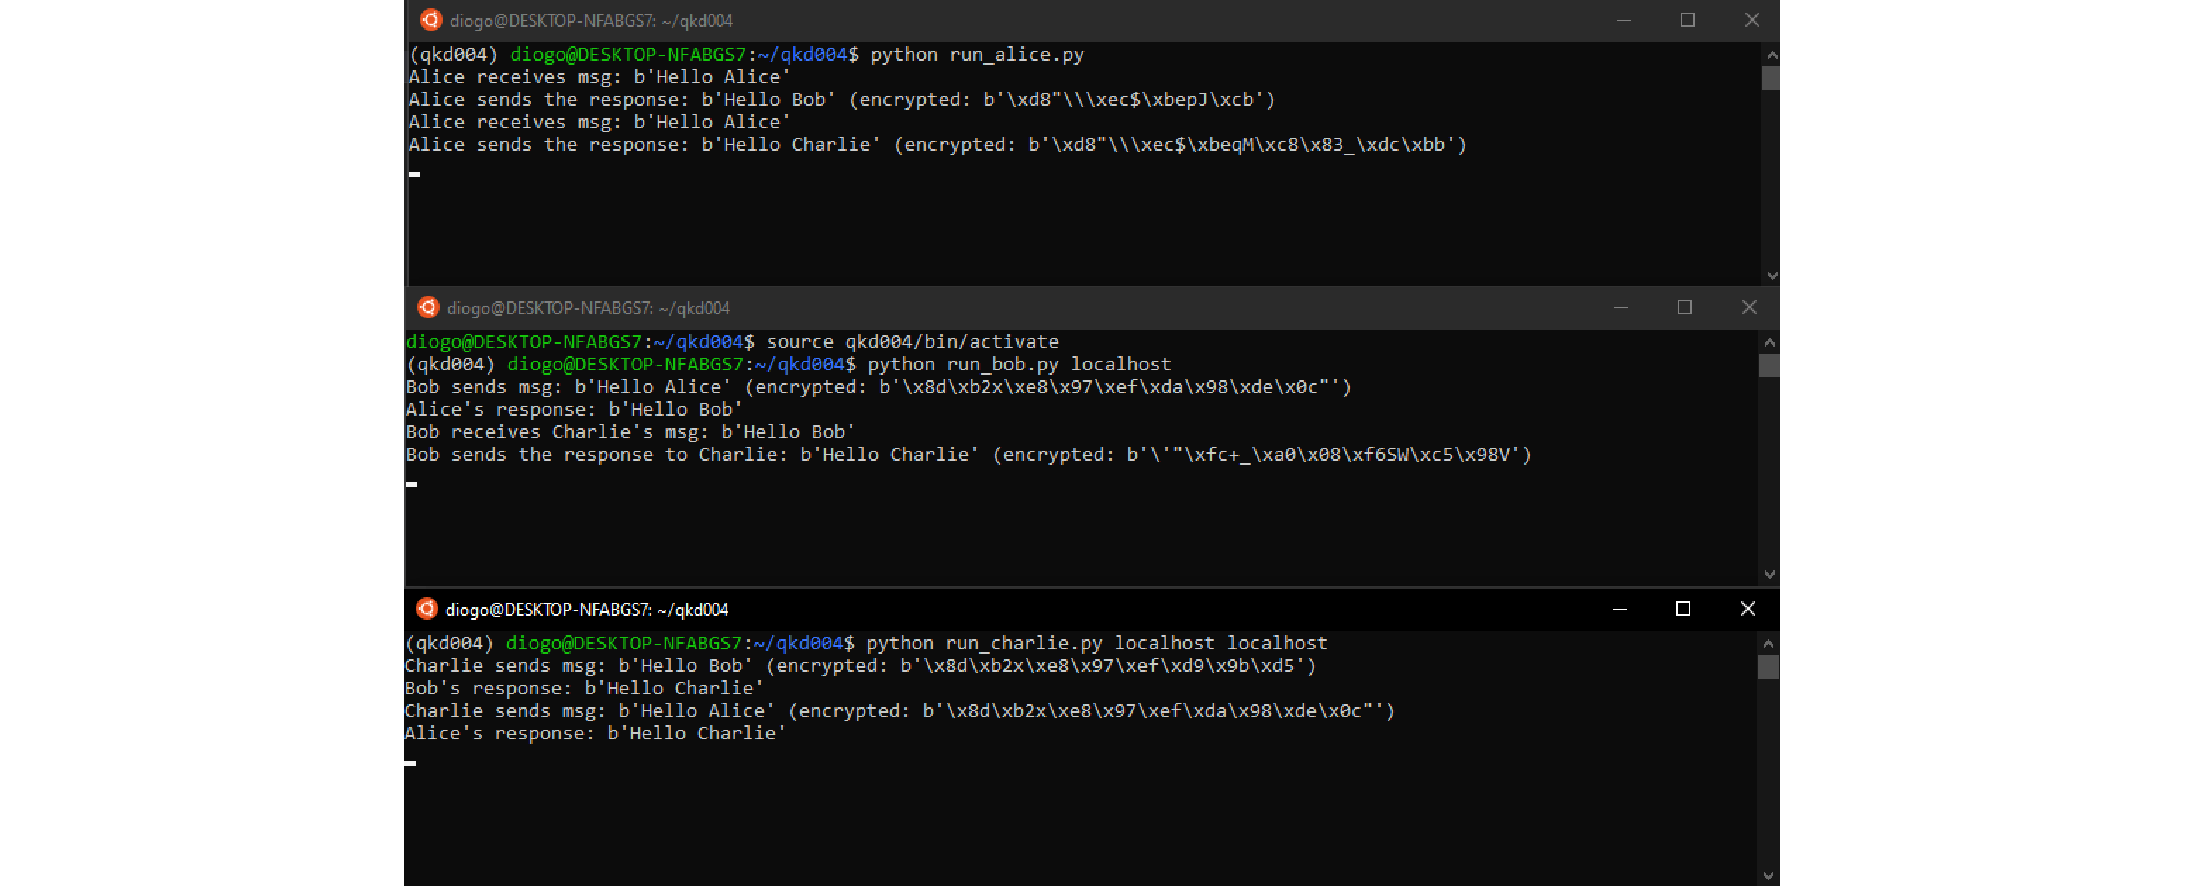
\includegraphics[width=15cm]{alicebobcharlie_example.pdf}
	\caption{Running the examples all on the same machine}
	\label{fig:3partyexample}
\end{figure}

\subsection{Raw Key Distribution}

\begin{figure}[H]
	\centering
	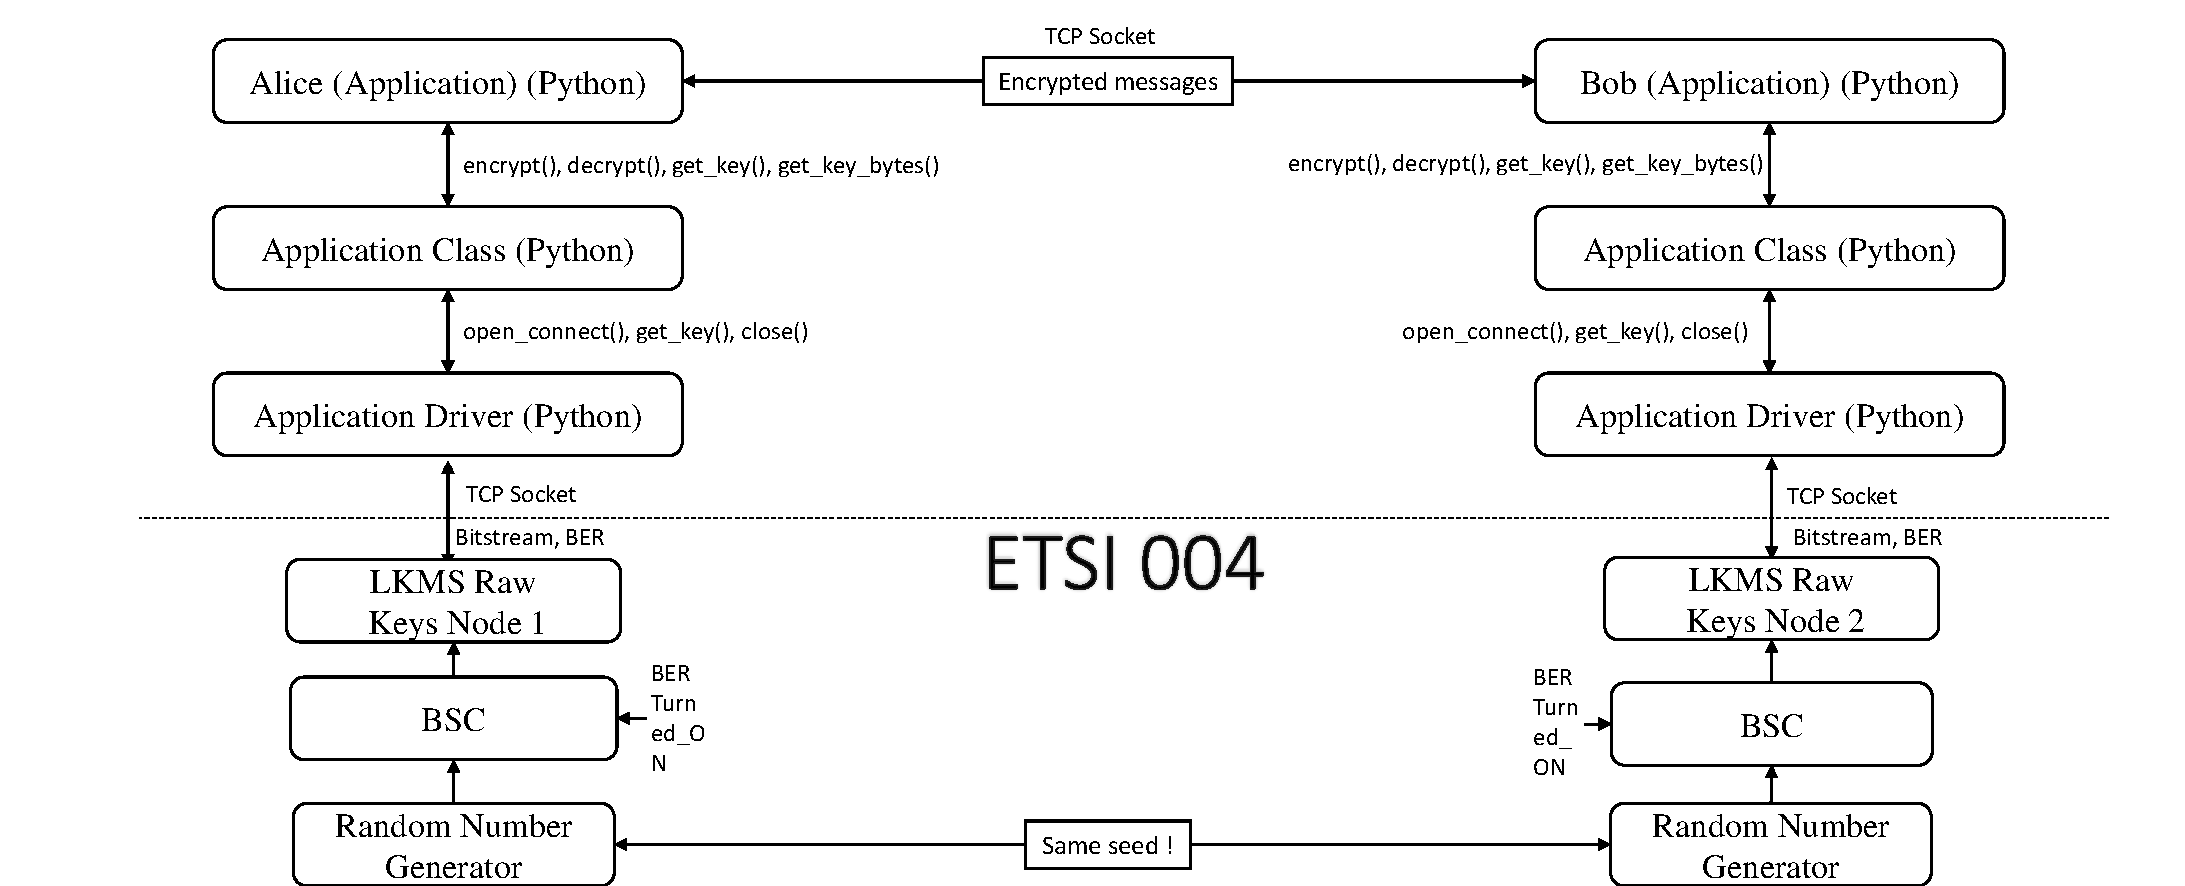
\includegraphics[width=15cm]{raw_key_distribution.pdf}
	\caption{Raw Key Distribution}
	\label{fig:rawkeydistribution}
\end{figure}

We have adapted the Madrid QKD example to also distribute raw keys. The way it works is when the LKMS Simulator is deployed, a seed and an error chance is associated with it. To deploy the LMKS use the following function:

\texttt{LKMSSimulator(("Address",Port),Seed,Error\textunderscore chance)}

The error chance should be an integer from 0 to 100

To connect to the Raw Key Manager you should use the same procedure as the symmetric key manager:

\texttt{app004 = App004(lkms\textunderscore address, source, destination, qos, KeyStreamId)}

The key can then be retrieved with:

\texttt{key = app004.get\textunderscore key\textunderscore bytes(size)}

An example called "test\textunderscore raw\textunderscore keys.py" is available in \texttt{/sdf/etsi\textunderscore qkd\textunderscore 004/qkd004/} 

\subsection{Development plan}

\begin{itemize}
	
	\item\underline{Socket Driver}

		Develop the socket driver, responsible for translating the API functions into bytes and parsing its responses.
		
		Classes:
		\begin{itemize}
			\item\underline{ksid}
			\item\underline{uri}
			\item\underline{qos}
			\item\underline{key\textunderscore buffer}
			\item\underline{metadata}
		\end{itemize}				
		
		Functions:
		\begin{itemize}
			\item\underline{openConnectRequest\textunderscore tobytes}
			\item\underline{openConnectRequest\textunderscore frombytes}
			\item\underline{openConnectResponse\textunderscore tobytes}
			\item\underline{openConnectResponse\textunderscore frombytes}
			\item\underline{getKeyRequest\textunderscore tobytes}
			\item\underline{getKeyRequest\textunderscore frombytes}
			\item\underline{getKeyResponse\textunderscore tobytes}
			\item\underline{getKeyResponse\textunderscore frombytes}
			\item\underline{closeRequest\textunderscore tobytes}
			\item\underline{closeRequest\textunderscore frombytes}
			\item\underline{closeResponse\textunderscore tobytes}
			\item\underline{closeResponse\textunderscore frombytes}
		\end{itemize}
	
	\item\underline{Application-KMS Driver Class}
		
		Create an Application driver class, responsible for storing and managing important information like QoS and KSID that can be used in its calls to the API using the Socket Driver.
		
		Attributes:
		\begin{itemize}
			\item\underline{kms\textunderscore address}
		\end{itemize}
		
		Methods:
		\begin{itemize}
		
			\item\underline{KmsDriver(address)}
		
				Application-Kms driver constructor	
		
			\item\underline{~KmsDriver}
		
				Application-Kms driver destructor
		
			\item\underline{void open\textunderscore connect(source, destination, qos, ksid, status)}
		
				Open Connect function
		
			\item\underline{void get\textunderscore key(ksid, index, metadata, status, key\textunderscore buffer)}
		
				Get Key function
		
			\item\underline{void close(ksid,status)}
		
				Close function
		
		\end{itemize}
		
	\item\underline{Application Class}
	
		Create an Application Class, responsible for abstracting the programmer from inner workings of the ETSI protocol, enabling him to provide the parameters and get the Key Buffer in return.
		
		Attributes:
		\begin{itemize}
			\item\underline{source}
			\item\underline{destination}
			\item\underline{qos}
			\item\underline{ksid}
			\item\underline{index}
			\item\underline{key\textunderscore buffer}
		\end{itemize}
		
		Methods:
		\begin{itemize}
			
			\item\underline{App004(address, source, destination, qos, ksid)}
		
				Application Class constructor	
		
			\item\underline{~App004}
		
				Application Class destructor
		
			\item\underline{keyBuffer get\textunderscore key(int size)}
		
				Gets key buffer as a KeyBuffer object
		
			\item\underline{char* get\textunderscore key\textunderscore bytes(int size)}
		
				Gets key buffer as an array of bytes
		
			\item\underline{char* encrypt(char* message)}
		
				Encrypts a message using XOR method
		
			\item\underline{char* decrypt(char* message)}
		
				Decrypts a message using XOR method
		
	\end{itemize}

	Example: 
	\begin{verbatim}
	#include <iostream>
	#include <string>
	#include "app_class.h"
	
	int main(){
		
		// LKMS Address and port
		
		std::string lkms_address = "192.168.1.100";
		uint32_t lkms_port = 44440;
		
		// Source and destination URI
		
		std::string source_uri =
		 "qkd://Application1@aaaaaaaa-aaaa-aaaa-aaaa-aaaaaaaaaaaa";
		std::string destination_uri =
		 "qkd://Application2@bbbbbbbb-bbbb-bbbb-bbbb-bbbbbbbbbbbb";
		
		// QoS - key_chunk_size, max_bps, min_bps, jitter, priority, ttl,
		// metadata_mimetype
		
		QoS qos = QoS(32,32,32,0,0,0,"raw+oblivious");
		
		// KSID
		
		std::string ksid = "12345678-1234-1234-1234-123456789012";
		
		// Initialize App class
		
		App004 alice_app = App004(lkms_address, lkms_port, source_uri,
		 destination_uri, qos, ksid);
		
		// Request a key from the App class
		
		char* key_buffer = alice_app.get_key_bytes(20, RAW_KEY);
		
		// Close connection
		
		alice_app.close()
		
	}		
	\end{verbatim}
	
		
\end{itemize}

\subsection{Madrid cpp 004 example}

\subsubsection{Introduction}

\begin{figure}[H]
	\centering
	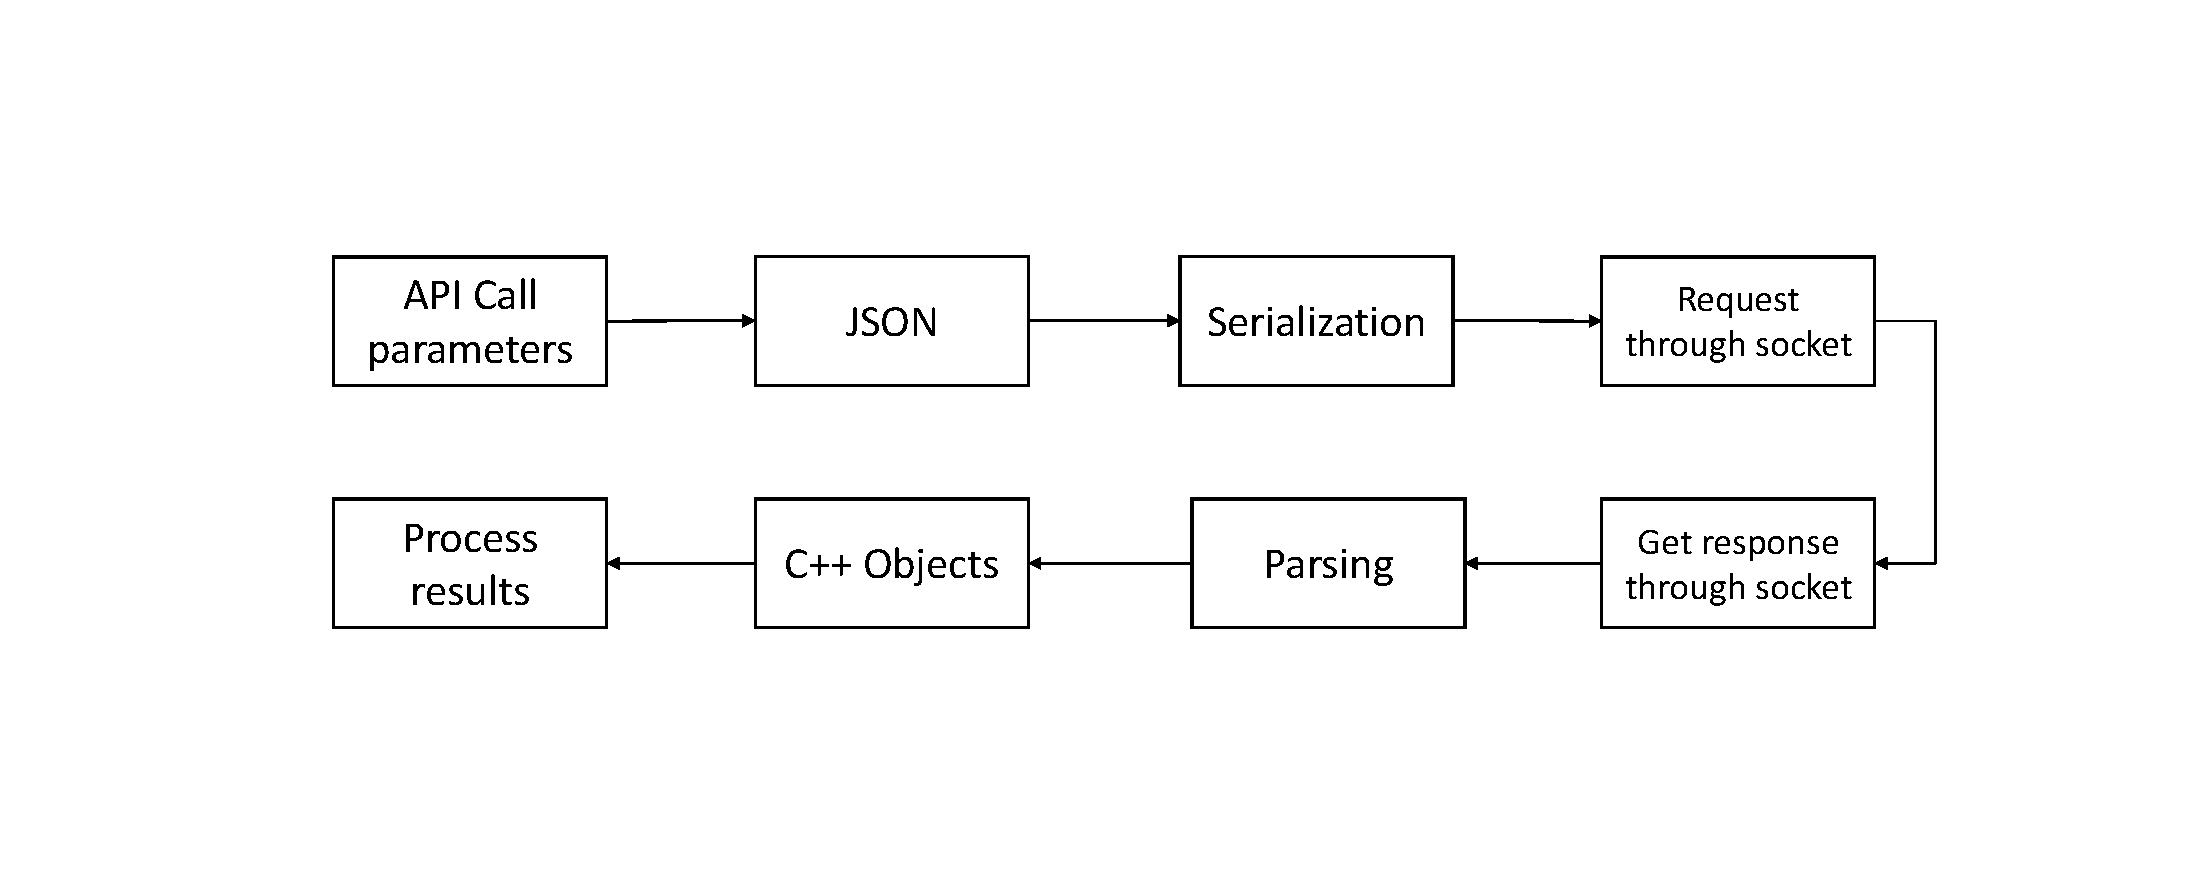
\includegraphics[width=15cm]{madrid_cpp.pdf}
	\caption{Madrid cpp example}
	\label{fig:madridcpp}
\end{figure}

The figure above tries to ilustrate how the cpp madrid example works. To start the API call parameters are defined. Once those parameters are defined (by the user), the API call function can be called. This function procedes to convert these parameters into a JSON object. The JSON object is then serialized and sent through a socket to the KMS. A response should be sent from the KMS through that same socket, which is then parsed and converted into a response struct and returned to the user that can then interpret these results as he wishes to.

\subsubsection{Example}

An example on how to use the madrid 004 cpp library was provided:

\begin{verbatim}
	#include <iostream>
	#include <nlohmann/json.hpp>
	#include "etsi_qkd_004.hpp"
	#include <stdexcept>
	#include <thread>
	
	void print_key_buffer(const etsi_qkd_004::KeyBuffer& key_buffer, 
	const std::string& name = "KEY BUFFER") {
		std::cout << name << ": [ ";
		std::for_each(key_buffer.cbegin(), key_buffer.cend(), 
		[](const unsigned char &c) { 
			std::cout << int(c) << " "; });
		std::cout << "]" << std::endl;
	}
	
	
	int main(int argc, char **argv) {
		if (argc - 1 != 2)
		throw std::invalid_argument("ERROR: Number of arguments " +
		std::to_string(argc - 1) +
		"\narg1 should be IP (ex: \"127.0.0.1\")"
		"\narg2 should be the PORT (ex: 1234)\n");
		
		etsi_qkd_004::LKMSAddress address = {argv[1], (unsigned short) atoi(argv[2])};
		std::cout << "Using address: " << address.ip << ':' 
		<< address.port << std::endl;
		
		// CONFIGURE DESIRED KEY (CHUNK_SIZE * CHUNK_NUMBER in bytes)
		// Number of key bytes retrieved per GET_KEY
		const unsigned int CHUNK_SIZE = 5;  
		// Number of key chunks you want to get
		const unsigned int CHUNK_NUMBER = 8;  
		
		// ----- OPEN_CONNECT -----
		// Classic key
		//    std::string source = "qkd:Application2@cccccccc-cccc-cccc-cccc-cccccccccccc";  
		// Classic key
		//    std::string destination = "qkd:Application1@bbbbbbbb-bbbb-bbbb-bbbb-bbbbbbbbbbbb";  
		// Raw key
		std::string source = "raw:Application2@cccccccc-cccc-cccc-cccc-cccccccccccc";  
		// Raw key
		std::string destination = "raw:Application1@bbbbbbbb-bbbb-bbbb-bbbb-bbbbbbbbbbbb";  
		
		etsi_qkd_004::QoS qos = {CHUNK_SIZE, 32, 32, 0, 0, 150000, 0, ""};
		auto oc_response = etsi_qkd_004::open_connect(address, 
		source, destination, qos);
		std::cout << "OPEN CONNECT STATUS: " << oc_response.status << std::endl;
		
		// ----- GET_KEY -----
		etsi_qkd_004::KeyBuffer cumulative_key_buffer;
		unsigned int index = 0;
		while (index < CHUNK_NUMBER) {
			std::this_thread::sleep_for(std::chrono::milliseconds(1000));
			auto gk_response = etsi_qkd_004::get_key(address, 
			oc_response.key_stream_id, index);
			if (gk_response.status == etsi_qkd_004::Status::SUCCESSFUL) {
				print_key_buffer(gk_response.key_buffer);
				
				// Extend cumulative_key_buffer
				cumulative_key_buffer.reserve(cumulative_key_buffer.size() +
				std::distance(gk_response.key_buffer.cbegin(),
				gk_response.key_buffer.cend()));
				cumulative_key_buffer.insert(cumulative_key_buffer.cend(),
				 gk_response.key_buffer.cbegin(),
				gk_response.key_buffer.cend());
				// Increment chunk index (only if gk_response.status is SUCCESSFUL)
				++index;
			}
			else
			;//std::cout << "ERROR: Status " << gk_response.status << std::endl;
		}
		print_key_buffer(cumulative_key_buffer, "CUMULATIVE KEY BUFFER");
		
		// ----- CLOSE -----
		auto cl_response = etsi_qkd_004::close(address, oc_response.key_stream_id);
		std::cout << "CLOSE STATUS: " << cl_response.status << std::endl;
		
		
		return 0;
	}
	
\end{verbatim}

This example can be found at sdf/etsi\textunderscore qkd\textunderscore 004/cpp/ .

It is important to note that the type of key requested is defined by the scheme in the URI.

To compile it use cmake:

\begin{verbatim}
	sudo apt-get install uuid-dev build-essential libssl-dev
	sudo snap install cmake --classic
	mkdir cmake-build
	cd cmake-build
	cmake ..
\end{verbatim}

\subsection{Requesting keys}

The type of keys requested are defined by the scheme in the URI. Example of QOKD URI: \texttt{"qokd:Application2@cccccccc-cccc-cccc-cccc-cccccccccccc"}.

Sample bytes received:

Alice: 10 10 10 00


Bob: 01 01 01 00

The first bit is the selection byte and the second one is the corresponding bit. 

To change the role played in QOKD use the role parameter in open\textunderscore connect. Example:

\begin{verbatim}
	std::string role = "bob";
	auto oc_response = etsi_qkd_004::open_connect(address, source, destination, qos,"b0dd24e6-94cb-4f32-abfe-50e194783a48", role);
\end{verbatim}


The system also provides symmetrical and raw keys:

\texttt{"qkd:Application2@cccccccc-cccc-cccc-cccc-cccccccccccc"}
\texttt{"raw:Application2@cccccccc-cccc-cccc-cccc-cccccccccccc"}


\subsection{Changing raw bit error rate}

To change the LKMS error rate edit the second parameter of LKMSSimulator on /sdf/etsi\textunderscore qkd\textunderscore 004/lkms/run\textunderscore lkms.py :

\begin{verbatim}
	def run_lkms_simulator(lkms_address):
		LKMSSimulator(lkms_address, 50)
\end{verbatim}


In this example the bit error rate is set to 50%

\subsection{How to get QKD, QOKD and RAW keys}

For the key delivery service to work we need two parts: the LKMS (Key Management Service) and the client.
The LKMS generates a different set of keys for each KSID (with the correct type, specified by the user). 
To start the LKMS execute \texttt{python3 run\textunderscore lkms.py} at \texttt{/sdf/etsi\textunderscore qkd\textunderscore 004/lkms/}. If you want to change the raw key error rate open 
the run\textunderscore lkms.py script and change the second argument of LKMSSimulator. Example of 50% error rate: 
\begin{verbatim}
	def run_lkms_simulator(lkms_address):
		LKMSSimulator(lkms_address, 50)
\end{verbatim}

After starting the LKMS Simulator it should be ready to provide keys. To test this you can use the example cpp program or write your own. The program is located in \texttt{/sdf/etsi\textunderscore qkd\textunderscore 004/cpp/}. If all is working then the cpp program should print out the keys provided by the LKMS. There are a couple of things that can be changed in the program:

\begin{itemize}
	\item\underline{KSID}
		You can provide your own KSID. In case you don't the LKMS should generate one and return it on the open\textunderscore connect call.

	\item\underline{Type of keys}
		The type of keys provided depends on the scheme of the source URI. Example:

		\texttt{"qkd:Application2@cccccccc-cccc-cccc-cccc-cccccccccccc"}
		\texttt{"raw:Application2@cccccccc-cccc-cccc-cccc-cccccccccccc"}

		The first one provides qkd keys and the second on raw. There are also qokd keys.

	\item\underline{Role of qokd keys}	

		To change the role (alice or bob) when getting qokd keys add a argument to the open\textunderscore connect function:

		\begin{verbatim}
			std::string role = "bob";
			auto oc_response = etsi_qkd_004::open_connect(address, source, destination
, qos,"b0dd24e6-94cb-4f32-abfe-50e194783a48", role);
		\end{verbatim}


\end{itemize}

To compile the example you first need to install the dependencies:
\begin{verbatim}
	sudo apt-get install uuid-dev build-essential libssl-dev
	sudo snap install cmake --classic
\end{verbatim}

After that go to the folder of the example:
\begin{verbatim}
mkdir cmake-build
cd cmake-build
cmake ..
make
\end{verbatim}
\subsection{Further Discussion}

\subsection{Open Issues}

\subsection{References}

\begin{itemize}
	\item
		ETSI GS QKD 004 V2.1.1 (2020-08)
\end{itemize}




\pagebreak


%%%%%%%%%%%%%%%%%%%%%%%%%%%%%%%%%%%%%%%%%%%%%%%%%%%%%%%%%%%%%%%%%%%%%%%%%%%%%%%%
% Acronyms
%%%%%%%%%%%%%%%%%%%%%%%%%%%%%%%%%%%%%%%%%%%%%%%%%%%%%%%%%%%%%%%%%%%%%%%%%%%%%%%%
\clearpage
\subsection*{Acronyms}\label{sec:acronyms}
\begin{acronym}[TDMA]
	\acro{DV-QKD}[DV-QKD]{Discrete Variables Quantum Key Distribution}
	\acro{QKD}[QKD]{Quantum Key Distribution}
\end{acronym}
\pagebreak 

%%%%%%%%%%%%%%%%%%%%%%%%%%%%%%%%%%%%%%%%%%%%%%%%%%%%%%%%%%%%%%%%%%%%%%%%%%%%%%%%
% References
%%%%%%%%%%%%%%%%%%%%%%%%%%%%%%%%%%%%%%%%%%%%%%%%%%%%%%%%%%%%%%%%%%%%%%%%%%%%%%%%

% bibliographic references for the section ----------------------------
\clearpage
\printbibliography[heading=subbibliography]
\end{refsection}
\addcontentsline{toc}{subsection}{Bibliography}
\cleardoublepage
% ---------------------------------------------------------------------

 \fi

%
% ------------------------------------------------------------------------
\chapter{Library}


%\input{./lib/adc/adc}
\input{./lib/add/add}
%\input{./lib/arithmetic_encoder/arithmetic_encoder}
%\input{./lib/arithmetic_decoder/arithmetic_decoder}
%\input{./lib/alice_incoming_data_processor/alice_incoming_data_processor}
%\input{./lib/alice_qkd/alice_qkd}
%\input{./lib/alice_qkd2/alice_qkd}
%\input{./lib/ascii_source/ascii_source}
%\input{./lib/ascii_to_binary/ascii_to_binary}
%\input{./lib/balanced_beam_splitter/balanced_beam_splitter}
\input{./lib/beam_splitter/beam_splitter}
%\input{./lib/bit_error_rate/bit_error_rate}
\input{./lib/binary_source/binary_source}
%\input{./lib/binary_to_ascii/binary_to_ascii}
%\input{./lib/bob_incoming_data_processor/bob_incoming_data_processor}
%\input{./lib/bob_qkd/bob_qkd}
%\input{./lib/bob_qkd2/bob_qkd}
%\input{./lib/BobQuantumRx/bobQRx}
%\input{./lib/decider/decider}
%\input{./lib/clock/clock}
%\input{./lib/clock_20171219/clock_20171219}
%\input{./lib/complex_to_real/complex_to_real}
%\input{./lib/coupler_2_by_2/coupler_2_by_2}
%\input{./lib/carrier_phase_estimation/carrier_phase_estimation}
%\input{./lib/decision_circuit/decision_circuit}
%\input{./lib/decoder/decoder}
\input{./lib/differential_photoreceiver/differential_photoreceiver}
\input{./lib/discrete_to_continuous_time/discrete_to_continuous_time}

\ifdefined\dvQkdCascade

\input{./lib/dv_qkd_basis_reconciliation/dv_qkd_basis_reconciliation}
\input{./lib/dv_qkd_error_correction/dv_qkd_error_correction}
\input{./lib/dv_qkd_message_processor_common/dv_qkd_message_processor_common}
\input{./lib/dv_qkd_message_processor_receiver/dv_qkd_message_processor_receiver}
\input{./lib/dv_qkd_message_processor_transmitter/dv_qkd_message_processor_transmitter}
\input{./lib/dv_qkd_parameter_estimation/dv_qkd_parameter_estimation}
\input{./lib/dv_qkd_privacy_amplification/dv_qkd_privacy_amplification}
\input{./lib/dv_qkd_rx/dv_qkd_rx}
\input{./lib/dv_qkd_rx_incoming_data_processor/dv_qkd_rx_incoming_data_processor}
\input{./lib/dv_qkd_rx_parameter_estimation/dv_qkd_rx_parameter_estimation}
\input{./lib/dv_qkd_tx/dv_qkd_tx}
\input{./lib/dv_qkd_tx_bases_reconciliation/dv_qkd_tx_bases_reconciliation}
\input{./lib/dv_qkd_tx_incoming_data_processor/dv_qkd_tx_incoming_data_processor}
\input{./lib/dv_qkd_tx_parameter_estimation/dv_qkd_tx_parameter_estimation}
\input{./lib/dv_polarization_physical_layer_emulator/dv_polarization_physical_layer_emulator}

\fi

\ifdefined\dvQkdLdpc

\input{./lib/dv_qkd_ldpc_rx_error_correction/dv_qkd_ldpc_rx_error_correction}
\input{./lib/dv_qkd_ldpc_tx_error_correction/dv_qkd_ldpc_tx_error_correction}
\input{./lib/dv_qkd_ldpc_tx_parameter_estimation/dv_qkd_ldpc_tx_parameter_estimation}
\input{./lib/dv_qkd_ldpc_rx_parameter_estimation/dv_qkd_ldpc_rx_parameter_estimation}
\input{./lib/dv_qkd_message_processor_transmitter_ldpc/dv_qkd_message_processor_transmitter_ldpc}
\input{./lib/dv_qkd_tx_ldpc/dv_qkd_tx_ldpc}

\fi

%\input{./lib/down_sampling/down_sampling}
%\input{./lib/dsp/dsp}
\input{./lib/electrical_filter/electrical_filter}
%\input{./lib/electrical_signal_generator/electrical_signal_generator}
\input{./lib/electro_optic_polarization_controller/electro_optic_polarization_controller}
%\input{./lib/entropy_estimator/entropy_estimator.tex}
%\input{./lib/error_correction/error_correction}
%\input{./lib/fork/fork}
\input{./lib/fiber/fiber}
%\input{./lib/gaussian_source/gaussian_source}
%\input{./lib/hamming_decoder/hamming_decoder.tex}
%\input{./lib/hamming_encoder/hamming_encoder.tex}
%\input{./lib/homodyne_receiver/homodyne_receiver.tex}
%\input{./lib/huffman_decoder/huffman_decoder.tex}
%\input{./lib/huffman_encoder/huffman_encoder.tex}
\input{./lib/ideal_amplifier/ideal_amplifier}
\input{./lib/ip_tunnel_linux/ip_tunnel_linux}
\input{./lib/ip_tunnel_ms_windows/ip_tunnel_ms_windows}
\input{./lib/iq_modulator/iq_modulator}
\input{./lib/laser/laser}
%\input{./lib/iir_filter/iir_filter}
%\input{./lib/local_oscillator/local_oscillator}
%\input{./lib/local_oscillator/local_oscillator_upgrade}
%\input{./lib/message_processors/message_processors}
%\input{./lib/mutual_information_estimator/mutual_information_estimator}
\input{./lib/mach_zehnder_modulator/mach_zehnder_modulator}
\input{./lib/m_qam_mapper/m_qam_mapper}
\input{./lib/m_qam_receiver/m_qam_receiver}
\input{./lib/m_qam_transmitter/m_qam_transmitter}
\input{./lib/ms_windows_console_output_common/ms_windows_console_output_common}
%\input{./lib/netxpto/netxpto}
\input{./lib/optical_amplifier/optical_amplifier}
%\input{./lib/alice_qkd/alice_qkd}
%\input{./lib/polarizer/polarizer}
%\input{./lib/probability_estimator/probability_estimator}
%\input{./lib/bob_qkd/bob_qkd}
%\input{./lib/eve_qkd/eve_qkd}
%\input{./lib/rotator_linear_polarizer/rotator_linear_polarizer}
%%\input{./lib/optical_attenuator/optical_attenuator}
%\input{./lib/ms_windows_ip_tunnel/ms_windows_ip_tunnel}
%\input{./lib/mutual_information_estimator/mutual_information_estimator}
%\input{./lib/optical_switch/optical_switch}
\input{./lib/optical_hybrid/optical_hybrid}
%\input{./lib/parameter_estimation/parameter_estimation}
\input{./lib/phase_modulator/phase_modulator}
\input{./lib/photodiode/photodiode}
\input{./lib/photodiode_pair/photodiode_pair}
%\input{./lib/photoelectron_generator/photoelectron_generator}
%\input{./lib/power_spectral_density_estimator/power_spectral_density_estimator}
%\input{./lib/privacy_amplification/privacy_amplification}
\input{./lib/pulse_shaper/pulse_shaper}
%\input{./lib/quantizer/quantizer}
%\input{./lib/quantum_channel_emulator_dv/quantum_channel_emulator_dv}
\input{./lib/quantum_bit_error_rate/quantum_bit_error_rate}
%\input{./lib/resample/resample}
%\input{./lib/snr_estimator/snr_estimator}
%\input{./lib/sampler/sampler}
%\input{./lib/snr_photoelectron_generator/snr_photoelectron_generator}
%\input{./lib/snr_estimator/snr_estimator}
%\input{./lib/single_photon_receiver/single_photon_receiver}
%\input{./lib/sop_modulator/sop_modulator}
%\input{./lib/source_code_efficiency/source_code_efficiency.tex}
%\input{./lib/white_noise/white_noise}
%\input{./lib/ideal_amplifier/ideal_amplifier}
%\input{./lib/phase_mismatch_compensation/phase_mismatch_compensation}
%\input{./lib/frequency_mismatch_compensation/frequency_mismatch_compensation}
%\input{./lib/cloner/cloner}
%\input{./lib/error_vector_magnitude/error_vector_magnitude}
%\input{./lib/load_ascii/load_ascii}
%\input{./lib/load_signal/load_signal}
%\input{./lib/matched_filter/matched_filter}
\input{./lib/transimpedance_amplifier/transimpedance_amplifier}
%\input{./lib/timing_deskew/timing_deskew}
%\input{./lib/dc_component_removal/dc_component_removal}
%\input{./lib/orthonormalization/orthonormalization}
%\input{./lib/interspace0s/interspace0s}
%\input{./lib/upsampler/upsampler}
%\input{./lib/resampler/resampler}
\input{./lib/sink/sink}
\input{./lib/subtractor/subtractor}
\input{./lib/white_noise/white_noise}








%
% ------------------------------------------------------------------------
\chapter{Mathlab Tools}

\input{./mtools/sgnToWfm/sgnToWfm}
\input{./mtools/polarizationAnalysis/polarizationAnalysis}

%
% ------------------------------------------------------------------------
\chapter{Algorithms}

\input{./algorithms/fourier_transform/fourier_transform}
\input{./algorithms/fft/fft}
\input{./algorithms/filter/filter}
\input{./algorithms/overlap_save/overlap_save}
\input{./algorithms/hilbert/hilbert}

%
% ------------------------------------------------------------------------
\chapter{Code Development Guidelines}

github.com/isocpp/CppCoreGuidelines/blob/master/CppCoreGuidelines.md

\subsection{Integrated Development Environment}

The recommended IDE is the Visual Studio 2017.
To install the Visual Studio 2017 first instal the Microsoft Visual Installer and after proceed to the Visual Studio 2017 installation.

\begin{tabular}{| l |}
\hline
Visual Studio Community 2017 - version 15.7.6 \\
\hline

\end{tabular}


\subsection{Compiler Switches}

\begin{tabular}{| l | l |}
\hline
Disable Language Extensions  & No \\
\hline
Conformance mode  & No \\
\hline
C++ Language Standard  & ISO C++14 Standard (std:c++ 14) \\
\hline
\end{tabular}








%\chapter{Building C++ Projects Without Visual Studio}

This is a guide on how to build C++ projects without having Microsoft Visual Studio installed.
All the necessary files will be available in the \textbackslash{}msbuild\textbackslash{} folder on this repository.


\section{Installing Microsoft Visual C++ Build Tools}
  Run the file \textbf{visualcppbuildtools\_full.exe} and follow all the setup instructions;
\section{Adding Path To System Variables}
  Please follow this step-by-step tutorial carefully.
  \begin{enumerate}
    \item Open the \textbf{Control Panel}.
    \item Select the option \textbf{System and Security}.
    \item Select the option \textbf{System}.
    \item Select \textbf{Advanced System Settings} on the menu on the left side of the window.
    \item This should have opened another window. Click on \textbf{Environment variables}.
    \item Check if there is a variable called \textbf{Path} in the \textbf{System Variables} (bottom list).
    \item If it doesn't exist, create a new variable by pressing \textbf{New} in \textbf{System Variables} (bottom list). Insert the name \textbf{Path} as the name of the variable and enter the following value \textbf{C:\textbackslash{}Windows\textbackslash{}Microsoft.Net\textbackslash{}Framework\textbackslash{}v4.0.30319}. Jump to step 10.
    \item If it exists, click on the variable \textbf{Path} and press \textbf{Edit}. This should open another window;
    \item Click on \textbf{New} to add another value to this variable. Enter the following value: \textbf{C:\textbackslash{}Windows\textbackslash{}Microsoft.Net\textbackslash{}Framework\textbackslash{}v4.0.30319}.
    \item Press \textbf{Ok} and you're done.
  \end{enumerate}
\pagebreak
\section{How To Use MSBuild To Build Your Projects}
  You are now able to build (compile and link) your C++ projects without having Visual Studio installed on your machine.
  To do this, please follow the instructions below:
  \begin{enumerate}
    \item Open the \textbf{Command Line} and navigate to your project folder (where the .vcxproj file is located).
    \item Enter the command:\\ \hbox{\textbf{msbuild <filename> /tv:14.0 /p:PlatformToolset=v140,TargetPlatformVersion=8.1,OutDir=``.\textbackslash{}''}} , where <filename> is your .vcxproj file.
  \end{enumerate}
  After building the project, the .exe file should be automatically generated to the current folder.\\
  The signals will be generated into the sub-directory \textbf{\textbackslash{}signals\textbackslash{}}, which must already exist.
\section{Known Issues}
  \subsection{Missing ucrtbased.dll}
  In order to solve this issue, please follow the instructions below:
  \begin{enumerate}
     \item Navigate to \textbf{C:\textbackslash{}Program Files (x86)\textbackslash{}Windows Kits\textbackslash{}10\textbackslash{}bin\textbackslash{}x86\textbackslash{}ucrt\textbackslash{}}
     \item Copy the following file: \textbf{ucrtbased.dll}
     \item Paste this file in the following folder: \textbf{C:\textbackslash{}Windows\textbackslash{}System32\textbackslash{}}
     \item Paste this file in the following folder: \textbf{C:\textbackslash{}Windows\textbackslash{}SysWOW64\textbackslash{}}
   \end{enumerate}
   \textbf{Attention}:you need to paste the file in BOTH of the folders above.

% ------------------------------------------------------------------------
\chapter{Git Helper}

\begin{refsection}

\section{Starting with Git}

Git is a free and open source distributed version control system~\cite{Chacon14}.
Git creates and maintains a database that records all changes that occur in a folder.
The Git database is named a repository.
It also allows to merge repositories that shared a common state in the past.
These can be local repositories, i.e. stored in the same machine, or can be remote repositores, i.e. stored anywhere.

To create this database for a specific folder the Git application must be installed on the computer.
The Git application and directions for its installation in all majors platforms can be obtained in the Git website (http://git-scm.com). You can access to the Git commands through the console or through a GUI interface.
Here, we assume that you are going to use the console.

After the installation, to create the Git initial database open the console program and go to a folder and execute the following command:
\\[0mm]
\par\textbf{git init}
\\[5mm]
The Git database is created and stored in the folder \emph{.git} in the root of your folder.
The \emph{.git} folder is your repository.

The Git commands allow you to manipulate this database, i.e. this repository.

\section{Data Model}

To understand Git is fundamental to understand the Git data model.

\begin{figure}[h!]
  \centering
  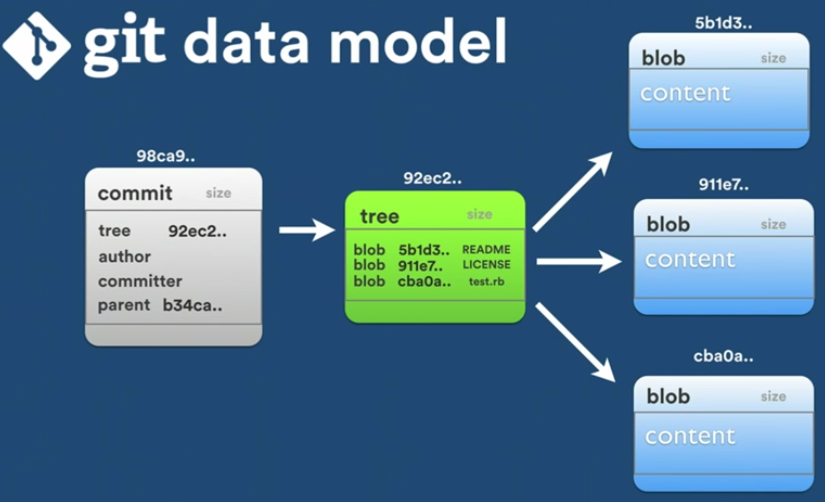
\includegraphics[width=12cm]{./chapter/git/figures/git_data_model.png}
  \caption{Git data model.}\label{git_data_model}
\end{figure}

Git manipulates the following objects:

\begin{itemize}
    \item[\textbullet] {commits - text files that store a description of the repository;}
    \item[\textbullet] {trees - text files that store a description of a folder;}
    \item[\textbullet] {blobs - the files that exist in your repository;}
    \item[\textbullet] {tags - text files that store information about commits.}
\end{itemize}
%
\noindent The objects are stored in the folder \emph{.git/objects}.
Each store object is identified by its SHA1 hash value, i.e. 20 bytes which identifies unequivocally the object.
The SHA1 is just an algorithm that accepts some binary information and generates 20 bytes which are ideally unique for that information. The probability of collisions is extremely low, i.e. the probability that different information generates the same hash value is extremely low.
Note that 20 bytes can be represented by a 40 characters hexadecimal string.
The identifier of each object is the 40 characters hexadecimal string.
Each particular object is stored in a sub-folder inside the \emph{.git/objects}.
The name of the sub-folder is the two most significative characters of the SHA1 hash value.
The name of the file that is inside the sub-folder is the remanning thirty eight characters of the SHA1 hash value.
The Git stores all committed versions of a file.
The Git maintains a contend-addressable file systems, i.e. a file system in which the files can be accessed based on its contend. Lets look more carefully in each stored object.

A \textbf{commit} object is identified by a SHA1 hash value, and has the following information: a pointer for a tree (the root), a pointer for the previous commit, the author, the committer and a commit message.
The author is the person who did the work. The committer is the person who validate the work and who apply the work by doing the commit. By doing this difference git allow both to get the credit, the author and the committer. Example of a commit file contend:\\
\\
tree 2c04e4bad1e2bcc0223239e65c0e6e822bba4f16\\
parent bd3c8f6fed39a601c29c5d101789aaa1dab0f3cd\\
author NetXPTO <netxpto@gmail.com> 1514997058 +0000\\
committer NetXPTO <netxpto@gmail.com> 1514997058 +0000\\
\\
Here goes the commit message.\\

A \textbf{tree} object is identified by a SHA1 hash value, and has a list of blobs and trees that are inside that tree.
A tree object identifies a folder and its contend.
Example of a tree file contend:\\
\\
\begin{tabular}{l l l l}
100644 & blob & bdb0cabc87cf50106df6e15097dff816c8c3eb34 &   .gitattributes\\
100644 & blob & 50492188dc6e12112a42de3e691246dafdad645b &   .gitignore\\
100644 & blob & 8f564c4b3e95add1a43e839de8adbfd1ceccf811 &   bfg-1.12.16.jar\\
040000 & tree & de44b36d96548240d98cb946298f94901b5f5a05 &   doc\\
040000 & tree & 8b7147dbfdc026c78fee129d9075b0f6b17893be &   garbage\\
040000 & tree & bdfcd8ef2786ee5f0f188fc04d9b2c24d00d2e92 &   include\\
040000 & tree & 040373bd71b8fe2fe08c3a154cada841b3e411fb &   lib\\
040000 & tree & 7a5fce17545e55d2faa3fc3ab36e75ed47d7bc02 &   msbuild\\
040000 & tree & b86efba0767e0fac1a23373aaf95884a47c495c5 &   mtools\\
040000 & tree & 1f981ea3a52bccf1cb00d7cb6dfdc687f33242ea &   references\\
040000 & tree & 86d462afd7485038cc916b62d7cbfc2a41e8cf47 &   sdf\\
040000 & tree & 13bfce10b78764b24c1e3dfbd0b10bc6c35f2f7b &   things\_to\_do\\
040000 & tree & 232612b8a5338ea71ab6a583d477d41f17ebae32 &  visualizerXPTO\\
040000 & tree & 1e5ee96669358032a4a960513d5f5635c7a23a90 &   work\_in\_progress\\
\end{tabular}
\\[5mm]

A \textbf{blob} is identified by a SHA1 hash value, and has the file contend compressed. A git header and tailor is added to each file and the file is compressed using the zlib library. The git header is just the object type, a space character, the file size in bytes and the \textbackslash NUL caracter, for instance "blob 13\textbackslash NUL", the tailor is just the \textbackslash n caracter. The compressed blob (header+file contend+tailer) is stored as a binary file.

There are two types of \textbf{tags}, lightweight and annotated tags. Lightweight tags are only a ref to a commit, see section below. Annotated tags are objects stored as text files, which as has information about the commit, to each the tag point, the tagger (name and e-mail), tag date and a tag message.

\subsection{Objects Folder}

Git stores the database and the associated information in a set of folders and files inside the the folder \emph{.git} in the root of your repository.

The folder \emph{.git/objects} stores information about all objects (commits, trees, blobs and annotated tags).
The objects are stored in files inside folders.
The name of the folders are the 2 first characters of the SHA1 40 characters hexadecimal string.
The name of the files are the other 38 hexadecimal characters of the SHA1.
The information is compressed to save space.

\section{Refs}

SHA1 hash values are hard to memorize by humans. To make life easier to humans we use refs. A ref associate a name, easier to memorize by humans, with a SHA1 hash value, used by the computer. Therefore refs are pointers to objects. Refs are implementes by text files, the name of the file is the name of the ref and inside the file is a string with the SHA1 hash value.
Tags and branches are example of refs. Tags are static references, i.e. tags are never updated, and branches are dynamic references, i.e. branches are always automatically updated.

\subsection{Refs Folder}

The \emph{.git/refs} folder has inside the following folders \emph{heads}, \emph{remotes}, and \emph{tags}.
The \emph{heads} has inside a ref for all local branches of your repository.
The \emph{remotes} folder has inside a set of folders with the name of all remote repositories, inside each folder is a ref for all branches in that remote repository.
The \emph{tag} folder has a ref for each tag.


\subsection{Branch}

A branch is a ref that points for a commit that is originated by a divergence from a common point.
A branch is automatically atualize so that it always points for the most recent commit of that branch.

\subsection{Heads}

Heads is a pointer for the branch where we are.
If we are in a commit that is not pointed by a branch we are in a detached HEAD situation.

\section{Git Logical Areas}

Git uses several spaces.

\begin{itemize}
    \item[\textbullet] {Working tree - is your directories where you are working;}
    \item[\textbullet] {Staging area or index - temporary area used to specify which files are going to be committed in the next commit;}
    \item[\textbullet] {History - recorded commits;}
\end{itemize}

All information related with the staging area and the history is stored in the \emph{.git} folder.

\begin{figure}[h!]
  \centering
  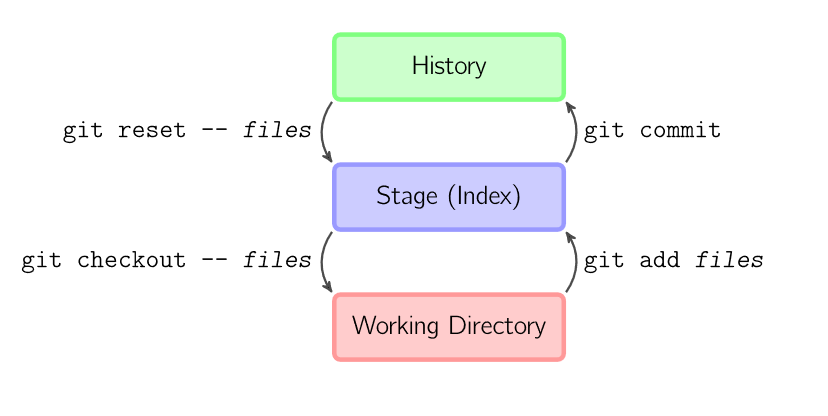
\includegraphics[width=12cm]{./chapter/git/figures/git_logical_areas.png}
  \caption{Git logical areas. Figure adapted from~\cite{Lodato19}.}\label{git_logical_areas}
\end{figure}

\section{Merge}

Merge is a fundamental concept to git. It is the way you consolidate your work.

\subsection{Fast-Forward Merge}

It is used when there is a direct path between the two branches, the older branch is just updated.

\subsection{Three-Way Merge}

It is used when there is no direct path between the two branches. In this case a common commit is found considering the two branches and the merge is performed using a recursive strategy.
In this process conflicts can occur.
The recursive strategy is applied to each modified file and line by line.
If the line was not modified in both branches the line is not modified in the merged file.
If the line was modified only in one branch the line is going to be modified in the merged file.
If the line is modified in both branches Git cannot make a decision and a conflict occur.
So, conflicts occur when branches that change the same file in the same line are being merged.

\section{Remotes}

A remote is a repository in another location. The remote location can be the http://github.com or the location of any other Git server.

\subsection{GitHub}

GitHub is a Git server that stores public repositories.
A GitHub user will have a user name and password and inside his or her account creates public repositories.
This repositories can be transferred to a local machine using the command \emph{git clone <repository url>}.
The local and remote repository will be linked and the local repository can be updated using the \emph{git fetch} or \emph{git pull} command.
The remote repository can be updated using the \emph{git push} command.
When the remote repository is cloned an alias, named origin, is created that points to that remote repository.
Another way to create a GitHub repository is by forking another existente repository.
Forked repositories are linked and they can be syncronized using pull requests.

\begin{figure}[h!]
  \centering
  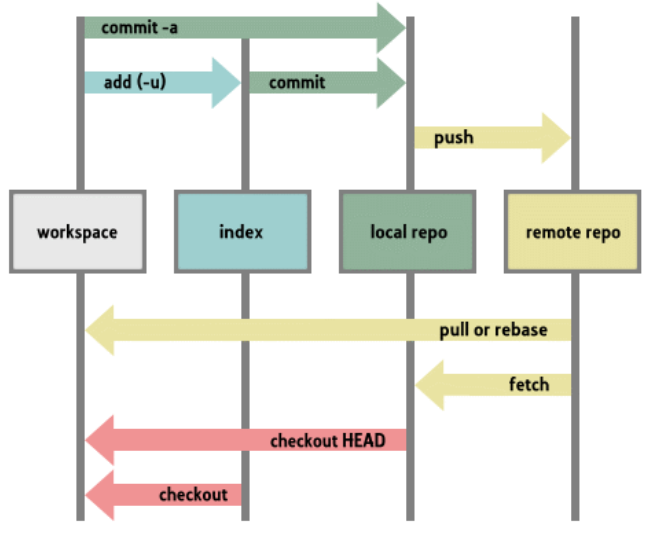
\includegraphics[width=12cm]{./chapter/git/figures/git_spaces.png}
  \caption{Git remotes.}\label{git_remotes}
\end{figure}

\section{Commands}


\subsection{Porcelain Commands}

Porcelain commends are high-level commands.

\vspace*{5mm} \noindent \textbf{git add}

\noindent \emph{git add}, adds a a new or modified file (or files) to the staging area.

\vspace*{5mm} \noindent \textbf{git branch}

\noindent \emph{git branch}, lists local branches.

\noindent \emph{git branch -r}, lists remote branches.

\noindent \emph{git branch -a}, lists all branches.

\noindent \emph{git branch -u <remote>/<branch>}, links the local branch in which you are in with a remote branch.

\noindent \emph{git branch --set-upstream-to=<remote>/<branch>}, longer version of the previous command.

\noindent \emph{git branch -u <remote>/<branch> <local\_branch>}, links the local branch with a remote branch.

\noindent \emph{git branch --set-upstream-to=<remote>/<branch> <local\_branch>}, longer version of the previous command.

\vspace*{5mm} \noindent \textbf{git cat-file}

\noindent \emph{git cat-file -t <hash>}, shows the type of the object identified by the hash value.

\noindent \emph{git cat-file -p <hash>}, shows the contend of the file associated with the object identified by the hash value.


\vspace*{5mm} \noindent \textbf{git checkout}

\noindent \emph{git checkout -b <new\_branch\_name>}, creates a new branch in the same position as the current branch and move to it.

\noindent \emph{git checkout -b <new\_branch\_name> <branch\_name>}, create a new branch in the position of <branch\_name> and move to it.

\vspace*{5mm} \noindent \textbf{git clean}

\noindent \emph{git clean -f -d}, removes from the working directory all untracked directories (d) and files (f).

\vspace*{5mm} \noindent \textbf{git clone}

\noindent \emph{git clone <url>}, downloads the contend of the <url> repository, for instance http://www.github.com/netxpto/linkplanner.git, and creates a local repo.

\vspace*{5mm} \noindent \textbf{git config}

\noindent \emph{git config --global user.name "netxpto"}, sets the user name globally.

\noindent \emph{git config --global user.email "netxpto.gmail.com"}, sets the user e-mail globally.

\noindent \emph{git config --global user.emmail "netxpto.gmail.com"}, sets the user e-mail globally.

\noindent \emph{git config --global alias.<alias name> <commands>}, creates a global alias for the commands.

\vspace*{5mm} \noindent \textbf{git diff}

\noindent \emph{git diff}, shows the changes between the working space and the staging area.

\noindent \emph{git diff --name-only}, shows the changes between the working space and the staging area, in the specified files.

\noindent \emph{git diff --cached}, shows the changes between the staging area and the current branch history. Note that --cached or --staged are synonymous.

\noindent \emph{git diff --cached --name-only}, shows the changes between the staging area and the current branch history, in the specified files.

\begin{figure}[H]
  \centering
  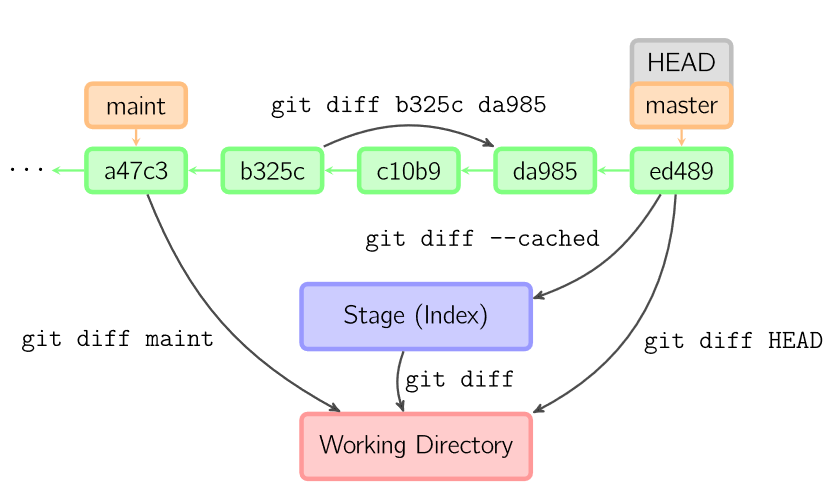
\includegraphics[width=12cm]{./chapter/git/figures/git_diff.png}
  \caption{Git diff command. Figure adapted from~\cite{Lodato19}.}\label{git_diff_command}
\end{figure}

\vspace*{5mm} \noindent \textbf{git fetch}

\noindent\emph{git fetch --all}, downloads all history from all remote repositories.

\noindent\emph{git fetch <repository>}, downloads all history from the remote repository.

\vspace*{5mm} \noindent \textbf{git init}

\noindent\emph{git init}, inicializes a git repository. It creates the \emph{.git} folder and all its subfolders and files.

\vspace*{5mm} \noindent \textbf{git log}

\noindent\emph{git log}, shows a list of commits from reverse time order.

\noindent\emph{git log --graph --decorate --oneline <commit1>..<commit1>}, shows the history of the repository in a colourful way.

\noindent\emph{git log --graph}, shows a graphical representation of the repository commits history.

\noindent\emph{git log --stat}, shows the name of the files that were changed in each commit

\noindent\emph{git log --follow <file>}, lists version history for a file, including rename.

\vspace*{5mm} \noindent \textbf{git ls-files}

\vspace*{5mm} \noindent \textbf{git ls-remote}

\vspace*{5mm} \noindent \textbf{git merge}

\noindent\emph{git merge <branch>}, combines the specified branch’s history into the current branch.

\vspace*{5mm} \noindent \textbf{git pull}

\noindent\emph{git pull}, downloads remote branch history and incorporates changes.

\vspace*{5mm} \noindent \textbf{git push}

\noindent\emph{git push}, uploads local branch commits to remote repository branch.

\vspace*{5mm} \noindent \textbf{git rebase}

\noindent\emph{git rebase <branch2 or commit2>}, finds a common point between the current branch and branch2 or commit2, reapply all commits of your current branch from that divergent points on top of branch2 or commit2, one by one.

\vspace*{5mm} \noindent \textbf{git remote}

\noindent\emph{git remote}, shows a list of existing remotes.

\noindent\emph{git remote -v}, shows the full location of existing remotes.

\noindent\emph{git remote add <remote name> <remote repository url>}, adds a remote.

\noindent\emph{git remote remove <remote name>}, removes a remote.

\vspace*{5mm} \noindent \textbf{git reset}

\noindent\emph{git reset --soft <commit\_hash\_value>}, moves to the commit identified by <commit\_hash\_value> but leaves in the staging area all modified files.

\noindent\emph{git reset --hard <commit\_hash\_value>}, moves to the commit identified by <commit\_hash\_value> and cleans all modified tracked files.

\noindent\emph{git reset <commit\_hash\_value>}, this is a mix reset (is the default reset), puts all modified files in the working area.

\noindent\emph{git reset <file>}, unstages the file, but preserve its contents.

\vspace*{5mm} \noindent \textbf{git reflog}

\noindent\emph{git reflog}, shows all commands from the last 90 days. Git only perform garbaged collection after 30 days.

\vspace*{5mm} \noindent \textbf{git rm}

\noindent\emph{git rm <file>}, deletes the file from the working directory and stages the deletion.

\noindent\emph{git rm --cached <file>}, removes the file from version control but preserves the file locally.

\vspace*{5mm} \noindent \textbf{git show}

\noindent\emph{git show}, shows what is new in the last commit.

\vspace*{5mm} \noindent  \textbf{git stash}

\noindent\emph{git stash}, temporarily stores all modified tracked files.

\noindent\emph{git stash --list}, shows what is in the stash.

\noindent\emph{git stash pop}, restores the most recently stashed files.

\noindent\emph{git stash drop}, discards the most recently stashed changeset.

\vspace*{5mm} \noindent \textbf{git status}

\noindent\emph{git status}, lists all new or modified files to be committed.

\subsection{Pluming Commands}

Pluming commands are low-level commands.

\vspace*{5mm} \noindent \textbf{git cat-files}

\noindent \emph{git cat-files -p <sha1>}, shows the contend of a file in a pretty (-p) readable format.

\noindent \emph{git cat-files -t <sha1>}, shows the type of a object, i.e. blob, tree or commit.

\vspace*{5mm} \noindent \textbf{git count-object}

\noindent \emph{git count-object -H}, counts all object and shows the result in a (-H) human readable form.

\vspace*{5mm} \noindent \textbf{git gc}

\noindent \emph{git gc}, garbage collector, eliminates all objects that has no reference associated with.

\noindent \emph{git gc --prune=all}


\vspace*{5mm} \noindent \textbf{git hash-object}

\noindent \emph{git hash-object <file>}, calculates the SHA1 hash value of a file plus a header.

\noindent \emph{git hash-object -w <file>}, calculates the SHA1 hash value of a file plus a header and write it in the \emph{.git/objects} folder.

\vspace*{5mm} \noindent \textbf{git merge-base}

\noindent \emph{git merge-base <branch1> <brach2>}, finds the base commit for the three-way merge between <branch1> and <branch2>.


\vspace*{5mm} \noindent \textbf{git update-index}

\noindent \emph{git update-index --add <file name>}, creates the hash and adds the <file\_name> to the index.

\vspace*{5mm} \noindent \textbf{git ls-files}

\noindent \emph{git ls-files --stage}, shows all files that you are tracking.

\vspace*{5mm} \noindent \textbf{git write-tree}

\vspace*{5mm} \noindent \textbf{git commit-tree}

\vspace*{5mm} \vspace*{5mm} \noindent \textbf{git rev-parse}

\noindent \emph{git rev-parse <ref>}, return the hash value of <ref>.

\noindent \emph{git rev-parse <short\_hash\_value>}, return the full hash value associated with <short\_hash\_value>.


\vspace*{5mm} \noindent \textbf{git update-ref}

\noindent \emph{git update-ref refs/heads/<branch name> <commit sha1 value>}, creates a branch that points to the <commit sha1 value>.

\vspace*{5mm} \noindent \textbf{git verify-pack}

\section{Navigation Helpers}

\noindent \emph{<ref>$^{\wedge}$}, one commit before <ref>.

\noindent \emph{<ref>$^{\wedge \wedge}$}, two commits before <ref>.

\noindent \emph{<ref>$\sim$5}, five commits before <ref>.

\noindent \emph{<ref1>..<ref2>}, between commit <ref1> and <ref2>.

\noindent \emph{<branch>$^{\wedge}${tree}}, identifies the tree pointed by the commit pointed by <branch>.

\noindent \emph{<commit>:<file\_name>}, identifies the version of a file in a given commit.

\section{Configuration Files}

There is a config file for each repository that is stored in the \emph{.git/} folder with the name \emph{config}.\\
\\
There is a config file for each user that is stored in the \emph{c:/users/<user name>/} folder with the name \emph{.gitconfig}.\\
\\
To open the \emph{c:/users/<user name>/.gitconfig} file type:\\
\\
\textbf{git config --global -e}

\section{Pack Files}

Pack files are binary files that git uses to save data and compress your repository. Pack files are generated periodically by git or with the use of gc command.

\section{Applications}

\subsection{Meld}

%# --------------------------------------D I F F -----------------------------
%
%[diff]
%    guitool = meld
%
%[difftool "meld"]
%    cmd = \"C:/Program Files (x86)/Meld/Meld.exe\" \"$LOCAL\" \"$REMOTE\" --label \"DIFF (ORIGINAL MY)\"
%	
%# --------------------------------------M E R G E -----------------------------
%
%[merge]
%    tool = meld
%
%[mergetool "meld"]
%    cmd = \"C:/Program Files (x86)/Meld/Meld.exe\" --auto-merge \"$LOCAL\" \"$BASE\" \"$REMOTE\" --output \"$MERGED\" --label \"MERGE (REMOTE BASE MY)\"
%    trustExitCode = false
%
%[mergetool]
%    # don't ask if we want to skip merge
%    prompt = false
%
%    # don't create backup *.orig files
%    keepBackup = false

\subsection{GitKraken}

\section{Error Messages}

\subsection{Large files detected}

Clean the repository with the \href{https://rtyley.github.io/bfg-repo-cleaner}{BFG Repo-Cleaner}.\\
\\
Run the Java program:\\

java -jar bfg-1.12.16.jar \texttt{-{}-}strip-blobs-bigger-than 100M\\
\\
This program is going to remote from your repository all files larger than 100MBytes. After do:\\

git push \texttt{-{}-}force.

\section{Git with Overleaf}

You can use git with overleaf.
For that you have to create a project on overleaf.
Associate with that overleaf project it is also create a git repository.
The address of that git repository is almost the same as the overleaf project that you can obtain going to the overleaf Menu/Share. Let's assume that the overleaf project address is:\\
\\
\noindent https://www.overleaf.com/12925162jkwbhrdkwrfm\\
\\
In this case the repository address is https://git.overleaf.com/12925162jkwbhrdkwrfm\\
%
The only change was the replacement of \textbf{www} by \textbf{git}.

Now you can just do

git clone https://git.overleaf.com/12925162jkwbhrdkwrfm

and clone your repository.

You can also do

git push https://git.overleaf.com/12925162jkwbhrdkwrfm


% bibliographic references for the section ----------------------------
\clearpage
\printbibliography[heading=bibliography]
\end{refsection}
\addcontentsline{toc}{section}{Bibliography}
\cleardoublepage
% ---------------------------------------------------------------------


%\chapter{Simulating VHDL Programs with GHDL}

This guide will help you simulate VHDL programs with the open-source simulator GHDL.

\section{Adding Path To System Variables}
Please follow this step-by-step tutorial:
  \begin{enumerate}
    \item Open the \textbf{Control Panel}.
    \item Select the option \textbf{System and Security}.
    \item Select the option \textbf{System}.
    \item Select \textbf{Advanced System Settings} on the menu on the left side of the window.
    \item This should have opened another window. Click on \textbf{Environment variables}.
    \item Check if there is a variable called \textbf{Path} in the \textbf{System Variables} (bottom list).
    \item \textbf{If it doesn't exist}, create a new variable by pressing \textbf{New} in \textbf{System Variables} (bottom list). Insert the name \textbf{Path} as the name of the variable and enter your absolute path to the folder \textbf{\textbackslash{}LinkPlanner\textbackslash{}ghdl\textbackslash{}bin}.\\ Example:
        \textbf{C:\textbackslash{}repos\textbackslash{}LinkPlanner\textbackslash{}ghdl\textbackslash{}bin}.\\
          Jump to step 10.
    \item \textbf{If it exists}, click on the variable \textbf{Path} and press \textbf{Edit}. This should open another window;
    \item Click on \textbf{New} to add another value to this variable. Enter your absolute path to the folder \textbf{\textbackslash{}LinkPlanner\textbackslash{}ghdl\textbackslash{}bin}.\\ Example:
        \textbf{C:\textbackslash{}repos\textbackslash{}LinkPlanner\textbackslash{}ghdl\textbackslash{}bin}.\\
    \item Press \textbf{Ok} and you're done.
  \end{enumerate}
\pagebreak
\section{Using GHDL To Simulate VHDL Programs}
This guide is meant to explain how to execute the testbench for module CPE BPS.\\
This simulation will take two .sgn files as input and produce two .sgn files.\\

\subsection{Simulation Input}
Make sure that files S19.sgn and S20.sgn exist in directory \textbf{\textbackslash{}LinkPlanner\textbackslash{}sdf\textbackslash{}dsp\_laser\_phase\_compensation\textbackslash{}signals}. The content of these files will be used as input of the CPE BPS module.

\subsection{Executing Testbench}
Execute the batch file \textbf{simulation.bat}, located in the directory \textbf{\textbackslash{}LinkPlanner\textbackslash{}sdf\textbackslash{}dsp\_laser\_phase\_compensation\textbackslash{}VHDL\textbackslash{}Simulator\textbackslash{}} of this repository.

\subsection{Simulation Output}
The simulation will produce two files: \textbf{sim\_out\_1.sgn} and \textbf{sim\_out\_2.sgn} which will contain the output of the CPE BPS module.

% -----------------------------------------------------------

\pagebreak

% -----------------------------------------------------------
%\bibliographystyle{ieeetr}
% argument is your BibTeX string definitions and bibliography database(s)
%\bibliography{../../../Computadores/Bibtex/IEEEabrv,../../../Computadores/Bibtex/AnpBib}
% -----------------------------------------------------------


%\printglossaries

\end{document}
